\documentclass[draft]{cmustatproposal} % remove draft option when done

\title{Texture encoding in the visual processing hierarchy}
\author{Al Xin}
\date{10 Dec 2026}

% Your advisor. If you have a coadvisor, just use \advisor twice.
% \advisor{Rob Kass}

% Your committee or external advisors. For external advisors or external
% committee members, be sure to include their affiliation.
\committee{Rob Kass, Statistics Advisor}
\committee{Jenelle Feather, External Advisor, CMU Psychology and Neuroscience Institute}

\documenttype{Advanced Data Analysis Project Report} % for ADA reports

% If your title is very long, it may not fit in the page headers. You can define
% a short version for those:
% \shorttitle{Your Title}

% The default font is Latin Modern, aka Computer Modern. You may choose a
% different font by uncommenting one of the following lines. All of these
% options include matching mathematics fonts.
% \usepackage{libertinus} % Libertinus (requires recent LaTeX from 2019 or newer)
% \usepackage{stix2} % STIX Two (also requires recent LaTeX)
% \usepackage{newtxtext,newtxmath} % Times New Roman style font
% \usepackage{newpxtext,newpxmath} % New PX, based on Palatino

% Put your custom commands here:
% For example,
% \DeclareMathOperator{\E}{\mathbb{E}}
% \DeclareMathOperator{\logit}{logit}

% Symbols %%%%%%%%%%%%%%%%%%%%%%%%%%%%%%%%%%%%%%%%%%%%%%%%%%%%%

\usepackage{amsthm}
\usepackage{amsmath}
\usepackage{amssymb}
\usepackage{amsfonts}

% New commands %%%%%%%%%%%%%%%%%%%%%%%%%%%%%%%%%%%%%%%%%%%%%%%%

% General mathematical symbols
% argmin help from egreg from tex.stackexchange.com/questions/5223
\newcommand{\R}{\mathbb{R}}
\newcommand{\onedim}{\mathbb{R}}
\newcommand{\ddim}{\mathbb{R}^d}
\newcommand{\kdim}{\mathbb{R}^k}

\newcommand{\eps}{\varepsilon}
\newcommand{\seq}[1]{\{ #1_{n} \}}
\newcommand{\bfs}[1]{\boldsymbol{ #1 }}

\DeclareMathOperator*{\sign}{sign}
\DeclareMathOperator*{\argmin}{arg\,min}
\DeclareMathOperator*{\argmax}{arg\,max}
\DeclareMathOperator*{\dist}{dist}
\DeclareMathOperator*{\diag}{diag}

% boldface
\newcommand{\bfX}{\mathbf{X}}
\newcommand{\bfx}{\mathbf{x}}
\newcommand{\bfY}{\mathbf{Y}}
\newcommand{\bfy}{\mathbf{y}}
\newcommand{\bfZ}{\mathbf{Z}}
\newcommand{\bfz}{\mathbf{z}}

% Sets
\newcommand{\setA}{\mathcal{A}}
\newcommand{\setB}{\mathcal{B}}
\newcommand{\setC}{\mathcal{C}}
\newcommand{\setF}{\mathcal{F}}
\newcommand{\rademacher}{\mathcal{R}}
\newcommand{\setP}{\mathcal{P}}

% General stats
\newcommand{\E}{\mathbb{E}}
\DeclareMathOperator*{\var}{Var}
\DeclareMathOperator*{\cor}{Corr}
\DeclareMathOperator*{\cov}{Cov}
\newcommand{\prob}{\mathbb{P}}

\newcommand{\indep}{\perp \!\!\! \perp}
\newcommand{\depen}{\cancel{\indep}}
\newcommand{\indic}{\mathbbm{1}}
\newcommand{\Xbar}{\overline{X}_n}
\newcommand{\Xsqbar}{\overline{X^2_n}}
\newcommand{\Xbarsq}{\overline{X}^2_n}
\newcommand{\Ybar}{\overline{Y}_n}
\newcommand{\lik}{\mathcal{L}}
\newcommand{\ton}[1]{#1_1, \dots, #1_n}
\newcommand{\fisher}{\mathcal{I}}
\newcommand{\sumn}{\sum_{i = 1}^n}
\newcommand{\prodn}{\prod_{i = 1}^n}

% Distributions
\newcommand{\hpp}{\textrm{HPP}}
\newcommand{\ipp}{\textrm{IPP}}
\newcommand{\geom}{\textrm{Geom}}
\newcommand{\iid}{\overset{\textrm{i.i.d.}}{\sim}}
\newcommand{\pois}{\textrm{Pois}}
\newcommand{\bern}{\textrm{Bern}}
\newcommand{\N}{\mathcal{N}}
\newcommand{\MVN}{\textrm{MVN}}
\newcommand{\unif}{\textrm{Unif}}
\newcommand{\binomial}{\textrm{Binom}}
\newcommand{\expo}{\textrm{Expo}}
\newcommand{\hgeom}{\textrm{HGeom}}


% Markup for TODFOs -----------------------------------------

\usepackage{xcolor}
\usepackage[normalem]{ulem} 
\usepackage{environ}        
\usepackage{tcolorbox}      
\usepackage{cancel} 
\tcbuselibrary{breakable, skins}

\usepackage{booktabs}

\newcommand{\todo}[1]{{\color{purple}#1}}
\newenvironment{todoblock}{\color{purple}}{}

%%%%%%%%%%%%%%%%%%%%%%%%%%%%%%%%%%%%%%%%%%%%%%%%%%%%%%%%%%%%%

\begin{document}
\maketitle

\begin{abstract}

\begin{todoblock}
!! Notes and temporary/uncertain text blocks in purple.

In object recognition, image information is first processed in the primary visual cortex (V1), then passes through V2, V4, and the inferotemporal cortex (IT). Later visual regions select for ``higher-level'' features. Outside of V1, the nature of these features remains ill-defined. For instance, previous work disagrees as to whether texture statistics remain well-encoded in IT. Natural textures are a special class of roughly homogeneous images that can be parameterized into families based on \( N \)th-order joint image densities. Higher between-family separability indicates that the recorded neurons select for the \(N\)th-order statistics that parameterize unique families. Previous work found better separability of texture families in V2 and V4 compared to V1 and lower family separability in IT compared to V4. However, IT tends to be sparser in both within-site responses and population responses. That is, individual neurons respond to only a few stimuli, and stimuli tend to evoke responses from only a few neurons. Thus, existing practices for correcting for sample size based on reliability tends to underestimate sparse sites in IT. When correcting these reliability cutoffs, we find that texture family separability consistently increases with each higher level region and that IT separability exceeds V4. Our results indicate that ``lower-level'' image features remain encoded in IT responses. That is, IT exhibits a sparse, ``efficient'' encoding of image features without necessarily summarizing over lower order statistics.
\end{todoblock}

\end{abstract}

\section{Introduction}

\begin{figure}
    \centering
    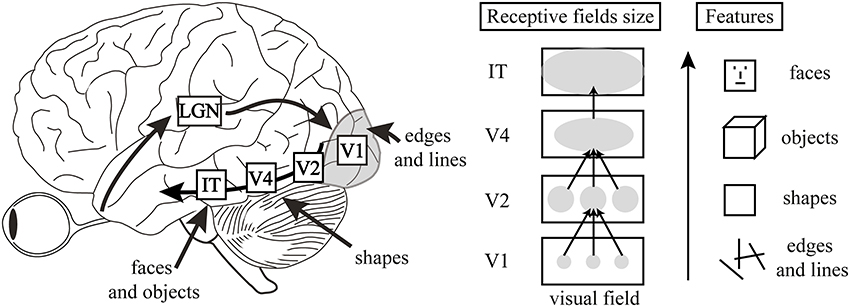
\includegraphics[width=0.7\linewidth]{img/eshuijs2023-visual_hierarchy.jpg}
    \caption{\todo{The regions involved in visual object recognition, copied from Eshuijs (2023) \cite{eshuijs_m31_2023} (TODO: replace with custom image for final presentation/report).}}
    \label{fig:visual_regions}
\end{figure}

After light hits the retina and initiates neural activity, the resulting image information passes through the primary visual pathway of the brain, producing the sensation of vision. Processing starts in the primary visual cortex (V1), then passes through V2, V4, and the inferotemporal cortex (IT).  Each subsequent area contains neurons selective for progressively ``higher-level'' visual features (Fig. \ref{fig:visual_regions}). For instance, neurons in V1 respond to simple oriented edges, while neurons in IT might respond to complex objects categories like hands or faces. 

However, relative  to V1, the response properties of neurons in various regions have not been well-defined. To discover relevant features, one can take a decoding approach. Given a diverse stimuli set, high separability of neural responses suggests selectivity for contrasting features in the set. Accordingly, low separability of responses suggests that differences in the stimuli are not well-represented. 

One approach to produce contrastive stimuli is with visual textures. Visual textures are approximately homogeneous images with repeated elements, such as sand, tree bark, granite, or honeycomb (Fig. \ref{fig:ex_texture}). Texture families can be parameterized by a set of image statistics, defined as \(N\)th-order empirical densities of pixels \cite{julesz_visual_1962, portilla_parametric_2000}. Furthermore, since image statistics are spatially averaged, textures in the same family can be visually distinct while sharing higher-order image statistics. Thus, by comparing responses to different families or unique images within families, one can determine whether the neurons select for the image statistics present in the provided textures.  

\begin{figure}
    \centering
    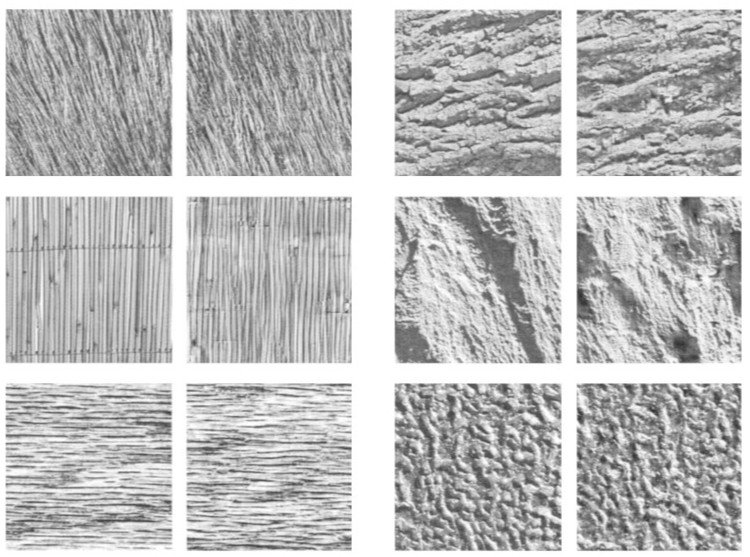
\includegraphics[width=0.5\linewidth]{img/portilla_simoncelli2000-textures.jpg}
    \caption{Example naturalistic textures, adapted from Figure 15 in Portilla and Simoncelli (2000) \cite{portilla_parametric_2000} \todo{(TODO: Replace with the real stimuli presented in the experiment).} For each pair, the left image was used as a seed to generate the statistics-matched images on the right.}
    \label{fig:ex_texture}
\end{figure}

Experiments with texture stimuli generally find that higher visual regions tend to be more selective for higher \(N\)th-order image statistics. Previously, Ziemba et al. (2016) found better within-family separation of neural responses in V1 and better between-family separation in V2 \cite{ziemba_selectivity_2016}. Furthermore, Okazawa et al. (2015, 2017) compared the selectivity of V2 and V4 neurons for image statistics in texture stimuli and found V4 neurons tended to be selective for higher order statistics \cite{okazawa_image_2015, okazawa_gradual_2017}. Other analyses of between-region texture responses found that texture stimuli with matched higher order image statistics produced higher firing of V2 and V4 neurons compared to stimuli lacking higher order image statistics  \cite{freeman_functional_2013, lee_developmentally_2024, lee_emergence_2025}. 

However, these existing analyses tend to lack results for the entire visual processing stream, with few experimenters recording textures responses in IT. Higher level areas tend to produce sparse responses, so typical approaches in the literature, such as size-matched population analyses or single-site neuron metrics, may not produce reliable comparisons between IT and earlier visual areas. \todo{(Tentative description) In IT, we found that neural responses to texture stimuli tend to be sparser than other regions, with a higher proportion of unreliable sites. When these differences are not accounted for, the separation of texture families appears greater in IT than V4. Surprisingly, within certain texture families, IT also achieves better separation of sample images, suggesting fine-grained image information remains represented in later visual areas.}

\section{Methods}

\todo{TODO: Add an overview.}

\subsection{Model of neural response separability}
In general, we can describe a site's response \( y \) to stimulus \( i \) at repetition \( r \) as 
\[ y_{i, r} = \mu + a_{i} + \epsilon_{i, r}, \]
where \( \mu \) is the site's baseline response (defined here as its response to a blank stimulus), \( a_i \) is the level effect of stimulus \( i \), and \( \epsilon_{i, r} (t) \) captures repetition-specific noise \( \epsilon \). \todo{Although the recorded neural response is a time series, we summarize the response by averaging/summing the firing over the response window (\ref{subsct:scalar_summary}).} 

By including family-wise and nested sample-wise effects, the model can be expanded as
\begin{equation}
\label{eqn:model}
% \mathbf{Y}_{f, s, r} (t) = \bfs{\mu}_{f, s} (t) + \bfs{\epsilon}_{f, s, r} (t)
y_{f, s, r} (t) = \mu + a_{f} + b_{s(f)} + c_r + \epsilon_{f, s, r},
\end{equation}
where \( f \in \{ 1, 2, \dots 35 \} \) indexes the texture family, \( s (f) \in \{ 1, 2, \dots, 15 \} \) indexes a sample image within family \( f \), and \( r \in \{ 1, 2, \dots, 6 \} \) indexes the repetition of a specific sample. Then, for a given region with \( p \) sites, we can write the population neural response as 
\begin{equation}
\label{eqn:model}
% \mathbf{Y}_{f, s, r} (t) = \bfs{\mu}_{f, s} (t) + \bfs{\epsilon}_{f, s, r} (t)
\mathbf{y}_{f, s, r} (t) = \bfs{\mu} + \mathbf{a}_{f} + \mathbf{b}_{s(f)} + \mathbf{c}_r + \bfs{\epsilon}_{f, s, r}, 
\end{equation}
where each term is a \( p \)-length vector. 

We can quantify the separability of the population neural response with Mahalanobis distance \(d_M: \mathbb{R}^p \times \mathbb{R}^p \to \mathbb{R} \) (Sec. \ref{methods:d_M}). We define the pairwise between-family separability as 
\[ d_M \left( \mathbf{a}_{f_1}, \mathbf{a}_{f_2}  \right) :  f_1 \neq f_2. \]
Within a fixed family \( f \), we define the pairwise between-sample separability as
\[ d_M \left( \mathbf{a}_{f} + \mathbf{b}_{s_1(f)}, \mathbf{a}_{f} + \mathbf{b}_{s_2(f)}  \right) : s_1 (f) \neq s_2 (f). \]
Mahalanobis distance is invariant to translation, so the grand mean \( \bfs{\mu} \) can be omitted from the separability definitions.


\subsection{Neural data collection}

\subsubsection{Texture stimuli synthesis and presentation}

Lee et al. (2024) generated texture stimuli with the Portilla and Simoncelli (PS) hierarchical parametric texture model. The lowest level of the model matches the local statistic of the original image, e.g., the correlation in luminance between adjacent pixels, the average luminance in a small area, or the total variation in luminance. Subsequent layers control higher level correlations, e.g., correlations between neighboring patterns of pixels. 
% Portilla and Simoncelli describe the higher levels as V1-like, or analogous to the receptive fields of the primary visual cortex.  
When synthesizing new samples from a seed image, matching the higher-level correlations produces \textit{naturalistic} structure, while omitting these statistics produces \textit{noise} texture (Fig. \ref{fig:noise_natur}). 

Lee et al. generated 15 samples of noise or naturalistic images from 35 families (\(15 \times 35 \times 2 = 1050\) unique images), with each family corresponding to a different original seed image. Within a session, Lee et al. presented 6 blocks of the 1050 images, with image order pseudorandomized within each block. Furthermore, to record baseline activity, each round contained 100 blank images, resulting in a total of \( 6 \times (1050 + 100) = 6900 \) observations per session. The experimenters presented images in blocks of 8 images, with each stimuli shown for 100 ms and followed by 100 ms of no stimulus. Presenting the stimuli in quick succession limits the recorded activity to short-term feed-forward visual processing rather than recurrent activity from longer-term cognitive processes. 
% The experimenters trained monkeys to fixate on the center of the screen and rewarded the monkeys for remaining fixated through a block.
% put this all in one experiment figure

\begin{figure}
    \centering
    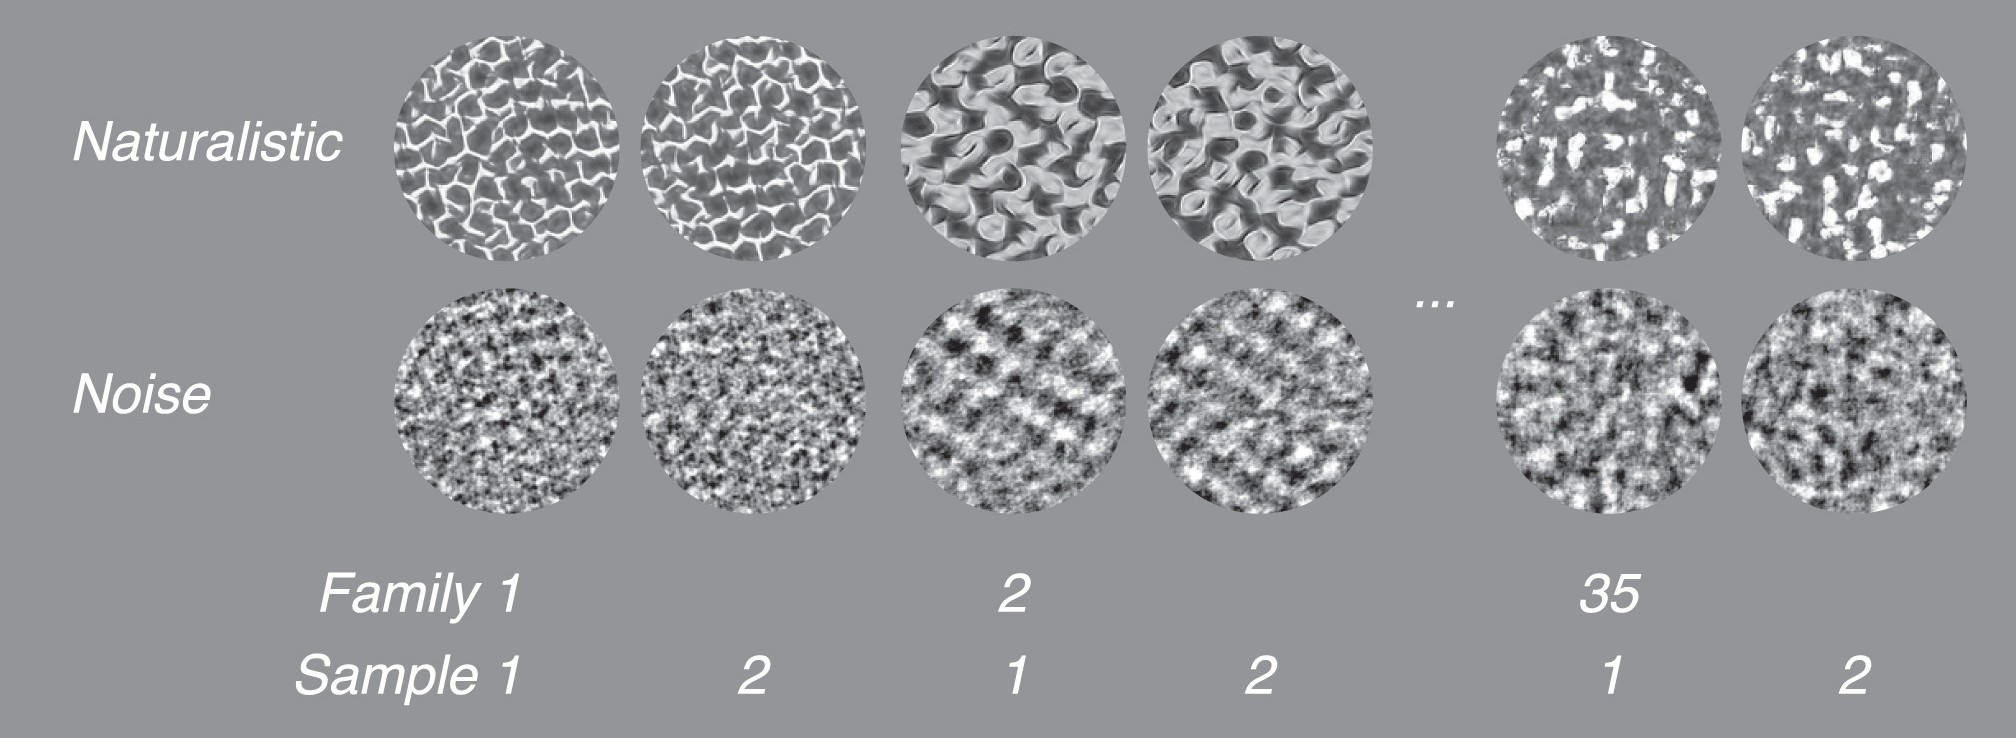
\includegraphics[width=0.8\linewidth]{img/lee2024-fig01-cropped.jpg}
    \caption{Naturalistic and noisy samples generated from different seed images, adapted from Figure 1 of Lee et al. (2024) \cite{lee_developmentally_2024}.}
    \label{fig:noise_natur}
\end{figure}

\subsubsection{Multi-unit activation recording}

\begin{table}[]
    \centering
    \small
    \begin{tabular}{cllllr}
    \toprule
        Region & Array 1 & Array 2 & Array 3 & Array 4 & Total  \\
    \midrule
        V1 & 61 (M1, 29) & 96 (M6, 36) &         &         & 157 \\
        V2 & 35 (M1, 29) & 96 (M2, 29) &         &         & 131 \\
        V4 & 96 (M1, 29) & 96 (M2, 29) & 96 (M8, 409) &         & 288 \\
        IT & 96 (M3, 20) & 96 (M6, 34) & 96 (M7, 34) & 96 (M6, 221) & 384 \\
    \bottomrule
    \end{tabular}
    \caption{The number of sites for each array for each region, with monkey ID and age of recording (in weeks) in parentheses. For M1, one array sat on the border between V1 and V2.}
    \label{tbl:sites}
\end{table}

Lee et al. (2024) chronically implanted six monkeys with two 96-site Utah arrays each. After surgery, the experimenters determined the array location based on anatomical landmarks and physiological response properties (see Table \ref{tbl:sites} for site numbers and locations). For each site, Lee et al. reported the \textit{multi-unit activations} (MUAs), defined as the number of times the voltage crossed some threshold within a 10 ms bin. MUAs reflect the combined activity of adjacent neurons, and up to ten neurons may contribute to the detected threshold crossings for a given site \cite{buzsaki_large-scale_2004}.

\subsection{Summarization of firing after response onset}
\label{subsct:scalar_summary}
% \begin{todoblock}
% (Delete this section for space?) Let \( i \in \{ 1, 2, \dots 35 \} \) index the texture family, \( j \in \{ 1, 2, \dots, 15 \} \) index the specific sample image, and \( k \in \{ 1, 2, \dots, 6 \} \) index the repetition of the specific image. Within a given array, the neural population response from \( p \) sites at time bin \( t \) can be modeled as
% \begin{equation}
%     \bfY_{i, j, k} (t) = \bfmu (t) + \bfX_{i, j} (t) + \bfeps_{i, j, k} (t), 
% \end{equation}
% where \( \bfY_{i, j, k} \in \mathbb{R}^p \) is a vector of the observed  responses, \( \bfmu \) is the vector of per-site mean responses, \( \bfX_{i, j} \) is the vector of expected neural responses to sample image \( j \) from family \( i \), and \( \bfeps_{i, j, k} \) is trial-specific noise \cite{pospisil_revisiting_2025} (\todo{replace this citation with a more basic methods paper}). For some distance metric \( d \), we are interested in the distributions of between-family distances \( d (\bfX_{i_1, -}, \bfX_{i_2, -}) : i_1 \neq i_2 \) and the between-sample distances \( d (\bfX_{i, j_1}, \bfX_{i, j_2}) : j_1 \neq j_2 \) \todo{which we estimate through inference on the observed \(\bfY_{i, j, k}\) (wording?)} 
% \end{todoblock}

For analyses, we summarized the MUAs by taking the mean firing rate in a 150 ms window after response onset.
% Due to biological constraints on neural signal propagation, the stimulus-response latency tends to increase for each successive region. 
We determined response onset with Lee et al.'s procedure \cite{lee_developmentally_2024}. For site \( s \) and bin \( t \), let the observed distance between non-blank and blank stimuli be
\begin{equation}
d'_s (t) = 
\frac{\mu_{\textrm{non-blank}} (t) - \mu_{\textrm{blank}} (t) }
{\sqrt{\frac{1}{2} \left( \sigma^2_{\textrm{non-blank}} (t) + \sigma^2_{\textrm{blank}} (t) \right)^2 }} \quad \textrm{(Cohen's d)},
\end{equation}
which can be estimated as
\begin{equation*}
\hat{d}'_s (t) = 
\frac{\overline{y}_{\textrm{non-blank}} (t) - \overline{y}_{\textrm{blank}} (t) }
{\sqrt{\frac{1}{2} \left( \hat\sigma^2_{\textrm{non-blank}} (t) + \hat\sigma^2_{\textrm{blank}} (t) \right)^2 }},
\end{equation*}
where \( \overline{y} \) is the mean across non-blank or blank stimuli and \( \hat\sigma^2 \) is the usual sample-corrected variance estimator. We can estimate the onset time for site \( s \) as the earliest \( t \) such that \( |\hat{d}'_s (t) |, |\hat{d}'_s (t + 1)|, |\hat{d}'_s (t + 2)| \geq 0.4 \) and share the same sign. For each region, we calculated the overall onset time as the median of estimated site onset times, giving an onset of 60 ms for V1, 70 ms for V2, 70 ms for V4, and 100 ms for IT (see Appendix \ref{appx:onsets}, Fig. \ref{fig:onsets} for details). \todo{TODO: These latencies are about 10-20 ms longer than reported in literature \cite{dicarlo_how_2012}, though shifting the windows earlier or shortening windows to 100 ms did not affect the overall results (Appendix \ref{appx:window}).}

\subsection{Reliability-based site selection between regions}

Distance calculations may be affected by a variety of features \todo{unrelated to the neural encoding of information}. For instance, the total number of recording sites varies by region (Table \ref{tbl:sites}) and higher dimensions can inflate the calculated distance. To address this, one could sub-sample a fixed number of sites from each region. However, this solution is imperfect, as sites are not necessarily independently sampled nor identically distributed. Sites within and between regions may differ in \textit{reliability}, \todo{defined as consistency in response to repetitions of the same stimulus.}

To measure site reliability, we calculated the split-half correlation on repetitions of the images. For each site, we split observations into two arbitrary groups of three repetitions each. We then averaged responses based on image then calculated the correlation between the splits (Pearson's \( r \)). To stabilize split-half correlation calculations, we averaged \( r \) over all \( \binom{6}{3} = 20 \) possible splits of two groups of three repetitions. We then obtained the reliability \( \rho \) by Spearman-Brown correcting the averaged correlations. Differences in handling blank images did not substantially affect the overall correlations, and correlations remained consistent over different choices of the split (Appendix \ref{appx:split_corrs}).  \todo{After matching site reliability, we sub-sampled \( p = 10, 20, 30, 40 \) sites for analyses.}

\subsection{Lifetime and population sparseness of sites}

Neural responses can exhibit \textit{lifetime} or \textit{population} sparseness \cite{willmore_characterizing_2001}. A single site shows lifetime sparseness if the responses are heavy-tailed, i.e., the site produces relatively large responses to a small set of stimuli. A group of sites shows population sparsity if only a small subset of neurons respond to any given stimulus, with the responsive subset varying based on stimulus. 

Let sites be indexed from \( s = 1, 2, \dots, p \) and let stimuli be indexed from \( i = 1, \dots, n \). Let \(\mu_{s, i} \geq 0 \) be site \( s \)'s mean response to the \(i\)th stimulus. Each site may exhibit different baseline firing rates, defined as the mean response to blank stimulus. For site \( s \), let \( \mu_{s, 0} \) be its baseline firing rate. To account for different baselines responses, we calculate sparsity on the log ratio of the responses, i.e., \( r_{s, i } = \log \left( \mu_{s, i} / \mu_{s, 0} \right) \). We can measure site \( s \)'s lifetime sparseness \( S_{s}^{L} \) with Hoyer sparsity \cite{hoyer_non-negative_2004}, calculated as
\begin{equation}
\label{eqn:sparsity_lifetime}
S_{s}^{L} = \frac{1}{\sqrt{n} - 1} \left( \sqrt{n} - \frac{\sum_{i = 1}^n |r_{s, i}|}{\sqrt{\sum_{i = 1}^n r_{s, i}^2}} \right),
\end{equation}
\todo{(TODO: possibly omit population sparseness).} Population sparseness \( S_{i, P} \) can be found similarly, but is instead taken with respect to the stimulus \( i \), i.e.,
\begin{equation}
\label{eqn:sparsity_population}
% S_{i, P} = \left( 1 - \frac{\left( \frac{1}{p} \sum_{s = 1}^p \mu_{i, s} \right)^2}{\frac{1}{p} \sum_{s = 1}^p \mu_{i, s}^2} \right) \left( \frac{1}{1 - \frac{1}{p}} \right).
S_{i, P} = \frac{1}{\sqrt{p} - 1} \left( \sqrt{p} - \frac{\sum_{s = 1}^p |r_{s, i}|}{\sqrt{\sum_{s = 1}^p r_{s, i}^2}} \right).
\end{equation}
The resulting sparsity values fall between \( [0, 1] \), where 0 corresponds to a uniform response distribution and 1 corresponds to a single non-zero response. For further discussion on different sparsity approaches, see Appendix \ref{appx:sparsity}.

% Alternatively, Hurley and Rickard (2009) suggest the Gini coefficient as an option that satisfies their desiderata for a sparseness metric \cite{hurley_comparing_2009}. On this dataset, we did not find substantial differences between the ratio of moments approach and the Gini coefficient (\todo{Appendix \ref{appx:sparsity_vs}}). 
\begin{todoblock}
% The above sparsity measure is invariant to multiplicative scaling but not translation. For instance, the addition of a positive constant to all observations reduces the calculated sparsity \cite{hurley_comparing_2009, dalton_measurement_1920}. Thus, we replaced raw firing rate with the deviation of the response from the baseline response (mean response to blank stimuli, ), i.e., \( | \Delta \mu_{i, s} | =  | \mu_{i, s} - \mu_{\textrm{blank}, s} |\). By taking the distance from the baseline, the sparsity measure reflects the sparseness of the site response \textit{to stimuli}. Then, when estimating lifetime sparsity, we first stabilized the observed responses by averaging over the six repetitions of each individual image, i.e., all pairwise combinations of of family \( i = 1, 2, \dots, 35 \) and sample \( j = 1, 2, \dots, 15 \). We estimated each site's \( \mu_{\textrm{blank}, s} \) by taking an average over the observed responses to blank images
% (TODO: Add figures demonstrating differences in baseline firing between regions and the spread of responses around the baseline.)
To estimate sparsity, we estimate the firing rate as \( \widehat\mu_{s, i} = \frac{1}{6} \sum_{k = 1}^{6} Y_{s, i, k} \), i.e., the observed mean of site \( s \)'s response to stimulus \( i \) over repetitions \( k = 1, 2, \dots, 6 \). Similarly, we estimate site \( s \)'s baseline response \( \widehat{\mu}_{s, 0} \) as site \( s \)'s observed mean over blank stimuli. Plugging these into the sparsity formula gives the estimator
\begin{equation}
\label{eqn:sparsity_estimate}
\hat{S}_{s}^{L} = \frac{1}{\sqrt{n} - 1} \left( \sqrt{n} - \frac{\sum_{i = 1}^n |\hat{r}_{s, i}|}{\sqrt{\sum_{i = 1}^n \hat{r}_{s, i}^2}} \right), \quad 
\hat{r}_{s, i} = \log \left( \frac{\widehat\mu_{s, i},}{ \widehat{\mu}_{s, 0}} \right)
\end{equation}
with \( \hat{S}_{i}^P \) defined similarly.

While the estimators \( \widehat\mu_{s, i}, \widehat{\mu}_{s, 0} \) may be individually unbiased, the estimator of sparsity will be biased due to Jensen's inequality. 
\end{todoblock}

\subsection{Separability based on Mahalanobis distance}
\label{methods:d_M}

% if you're wondering why this is suddenly \pmb instead of \boldsymbol or \mathbf, it's because \pmb is the only one that works with \Sigma

% \begin{todoblock}
% (Possibly delete for space) 
% To characterize separability of responses, we applied the the Mahalanobis distance. In general, let \( P \) be some probability distributions on \( \mathbb{R}^k \) with mean \( \pmb{\mu} \) and covariance matrix \( \pmb\Sigma \). The Mahalanobis distance of points \( \bfx, \bfy \) with respect to \( P \) is
% \begin{equation}
% d_M (\bfx, \bfy, P) = 
% \sqrt{ ( \bfx - \bfy )^\intercal \pmb\Sigma^{-1} ( \bfx - \bfy ) }.
% \end{equation}
% If \( \pmb{\Sigma} \) is positive semi-definite, the covariance can be decomposed as \( \pmb\Sigma = \mathbf{S}^\intercal \mathbf{S} \), where \( \mathbf{S} \) is the standard deviation matrix. So, the Mahalanobis distance is equivalently 
% \[ d_M (\bfx, \bfy, P) = \| \mathbf{S}^{-1} (\bfx - \bfy) \|, \]
% or the Euclidean distance after a whitening transformation. 
% \end{todoblock}

\todo{(TODO: Rewrite with notation specific to this problem to avoid introducing \( \bfx, \bfy \).)}
To estimate the separability of neural responses, we calculated the Mahalanobis distance \( d_M \) as applied in Hotelling's two-sample \( t \)-test.  
% Let $P \sim \mathcal{N}_k (\pmb\mu, \pmb\Sigma)$, i.e., a $k$-dimensional multivariate Normal distribution. 
% it would be more consistent to use d for the number of sites
% but it collides with d_M
Generally, let \( P \) be some distribution on \( \mathbb{R}^p \) and take \( \bfx_1, \bfx_2, \dots, \bfx_{n_x} \) and \( \bfy_1, \bfy_2, \dots, \bfy_{n_y} \) as independent samples from \( P \). Let each sample be a column vector. We can then define the sample mean vectors
\( \overline{\bfx} = \frac{1}{n_x} \sum_{i = 1}^{n_x} \bfx_i,
\overline{\bfy} = \frac{1}{n_y} \sum_{i = 1}^{n_y} \bfy_i, \)
and the sample covariance matrices
\[ 
\hat{\pmb\Sigma}_{\bfx} = \frac{1}{n_x - 1} \sum_{i = 1}^{n_x} (\bfx_i - \overline\bfx) (\bfx_i - \overline\bfx)^\top, \quad
\hat{\pmb\Sigma}_{\bfy} = \frac{1}{n_y - 1} \sum_{i = 1}^{n_y} (\bfy_i - \overline\bfy) (\bfy_i - \overline\bfy)^\top. 
\]
The unbiased pooled covariance matrix estimate is the weighted average of the sample covariance matrices 
\( \hat{\pmb\Sigma} = \frac{1}{n_x + n_y - 2} \left( 
(n_x - 1) \hat{\pmb\Sigma}_{\bfx} + (n_y - 1) \hat{\pmb\Sigma}_{\bfy} \right), \)
and the Mahalanobis distance can be found as
\begin{equation}
d_M (\bfx, \bfy, P) = 
\sqrt{ (\overline{\bfx} - \overline{\bfy})^\top \hat{\pmb\Sigma}^{-1} (\overline{\bfx} - \overline{\bfy}) }.
\end{equation}
If \( \hat{\pmb\Sigma} \) is positive semi-definite, the covariance can be decomposed as \( \hat{\pmb\Sigma} = \hat{\mathbf{S}}^\top \hat{\mathbf{S}} \), where \( \hat{\mathbf{S}} \) is the estimated standard deviation matrix. So, the Mahalanobis distance is equivalently 
\( d_M (\overline{\bfx} - \overline{\bfy}) = \| \hat{\mathbf{S}}^{-1} (\overline{\bfx} - \overline{\bfy}) \|, \)
or the Euclidean distance after a whitening transformation. Thus, \( d_M \) is invariant to linear transformation like centering and scaling and automatically normalizes between-site differences in mean firing rate or variance. 

\subsubsection{Shrinkage covariance estimation}

For between-sample comparisons, the standard multivariate covariance estimator cannot be applied in \( d_M \) because the number of repetitions (\( n = 6 \)) is lower than the number of sites \( p \). However, one can apply a shrinkage approach, described in Schafer and Strimmer \cite{schafer_shrinkage_2005} and based on a lemma proposed by Ledoit and Wolf  \cite{ledoit_improved_2003}. This approach is implemented in the R package \texttt{corpcor} \cite{schafer_corpcor_2021} and briefly described in Appendix \ref{appx:shrinkage}.

\section{Results}

\subsection{Reliable IT sites tend to be sparser}

Split-half correlations in V1 and IT were right-skewed, with a mode of \( \rho \approx 0.1 \). For V2, the correlations were left-skewed. V4 has a somewhat bimodal distribution, with a local peak of \( \rho \approx 0.1 \) and \( \rho \approx 0.6 \) (Figure \ref{fig:split_corrs_distribution}). Among reliable sites of \( \rho > 0.2 \), the distribution of per-site lifetime sparsities \(S^\textrm{lifetime} \) tended to be lower and more concentrated for V1. The distributions looked more similar between V2, V4, and IT, with IT slightly higher (Figure \ref{fig:sparsity_vs_corr}, top). Reliable sites in IT tended to be sparser, and unlike other regions, IT lacked reliable sites with \textit{low} sparsity (Figure \ref{fig:sparsity_vs_corr}, bottom). 

\todo{(TODO: High sparsity sites in V2 and V4 show qualitative differences from high sparsity sites in IT. Namely, more consistency in firing within families).}

\begin{figure}
    \centering
    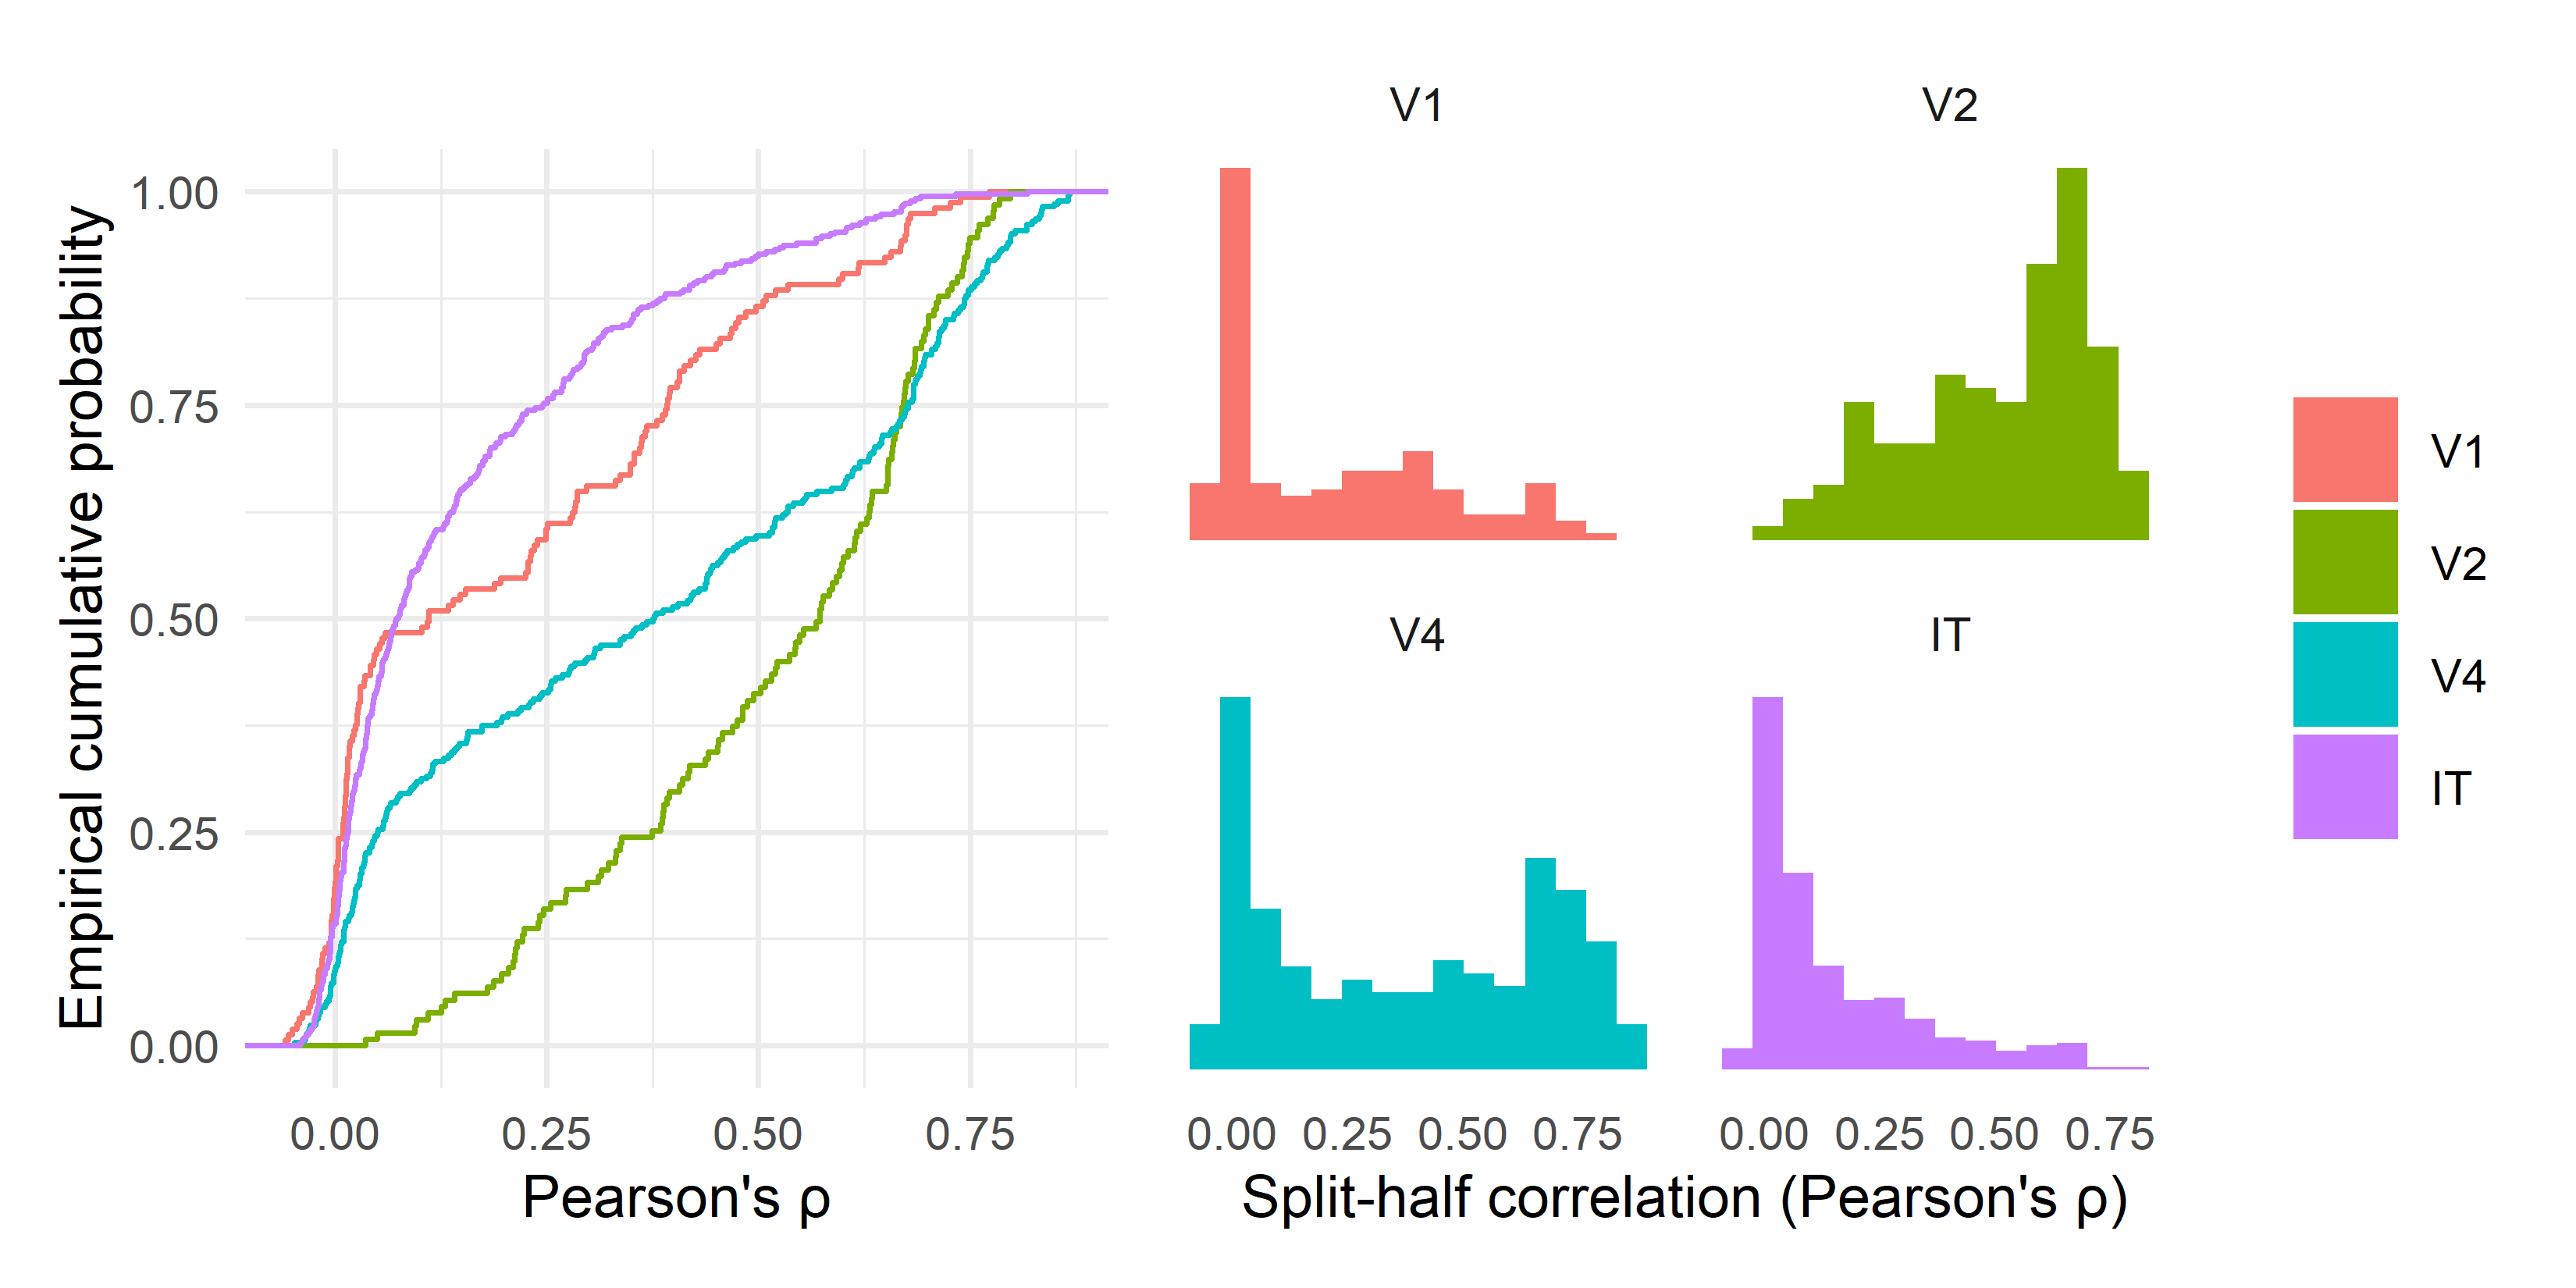
\includegraphics[width=0.9\linewidth]{img/split_corrs_distribution.png}
    \caption{(Left) Empirical cumulative distribution functions. (Right) Histograms for the split-half correlations by region. Data reflects split-half correlations performed when all blanks are averaged. V1 and IT are right-skewed, V2 is left-skewed, and V4 has a somewhat bimodal distribution for low- and high-correlations.}
    \label{fig:split_corrs_distribution}
\end{figure}

\begin{figure}
    \centering
    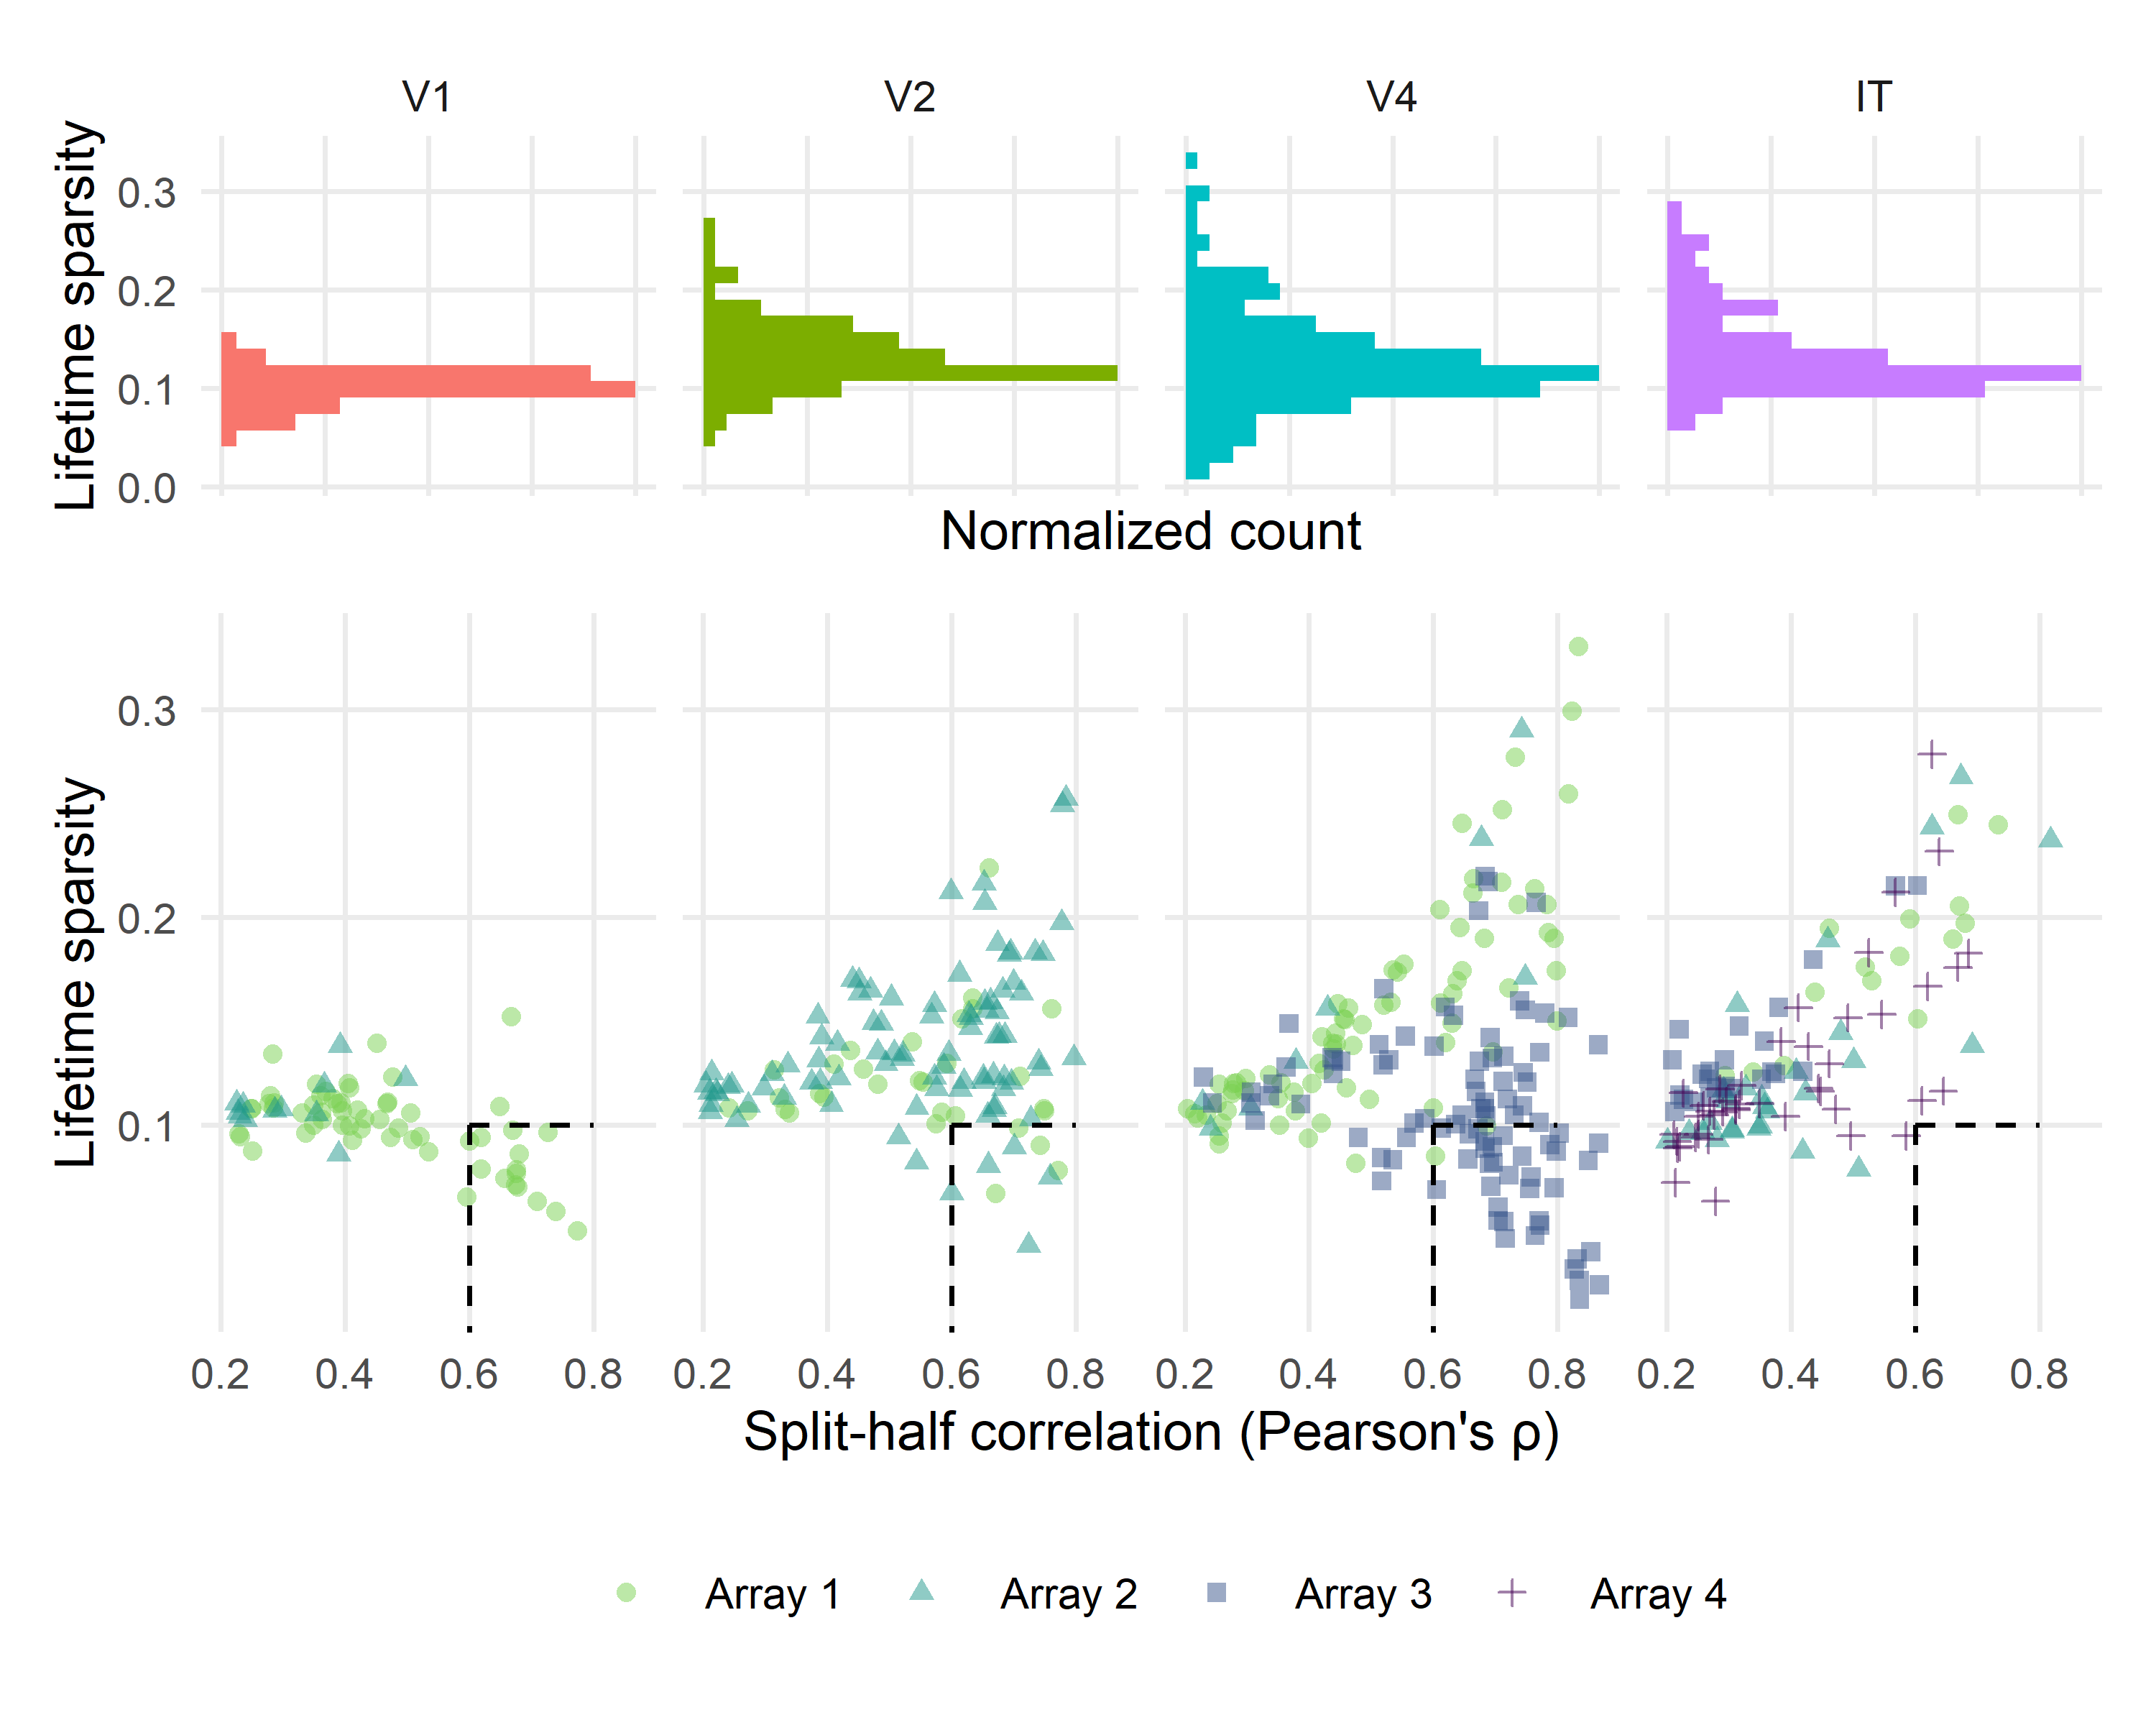
\includegraphics[width=0.8\linewidth]{img/sparsity_vs_corr.png}
    \caption{(Top) Height-normalized histograms of lifetime (per-site) sparsities for each region, only including sites with \( \rho > 0.2 \). (Bottom) Lifetime sparsity and split-half correlation, with within-region arrays separated by color and shape. The dashed lines in the lower right covers sites with low sparsity (\(S^\textrm{lifetime}_s < 0.1 \) and high reliability (\( \rho > 0.6 \)). }
    \label{fig:sparsity_vs_corr}
\end{figure}

\subsection{IT responses show sparseness at the sample level, not the family level}

\todo{TODO: Write up Figure \ref{fig:sparsity_fam_vs_img}. Also, need to append the baseline firings and average firings to the figure to make argument more obvious.}

\begin{figure}
    \centering
    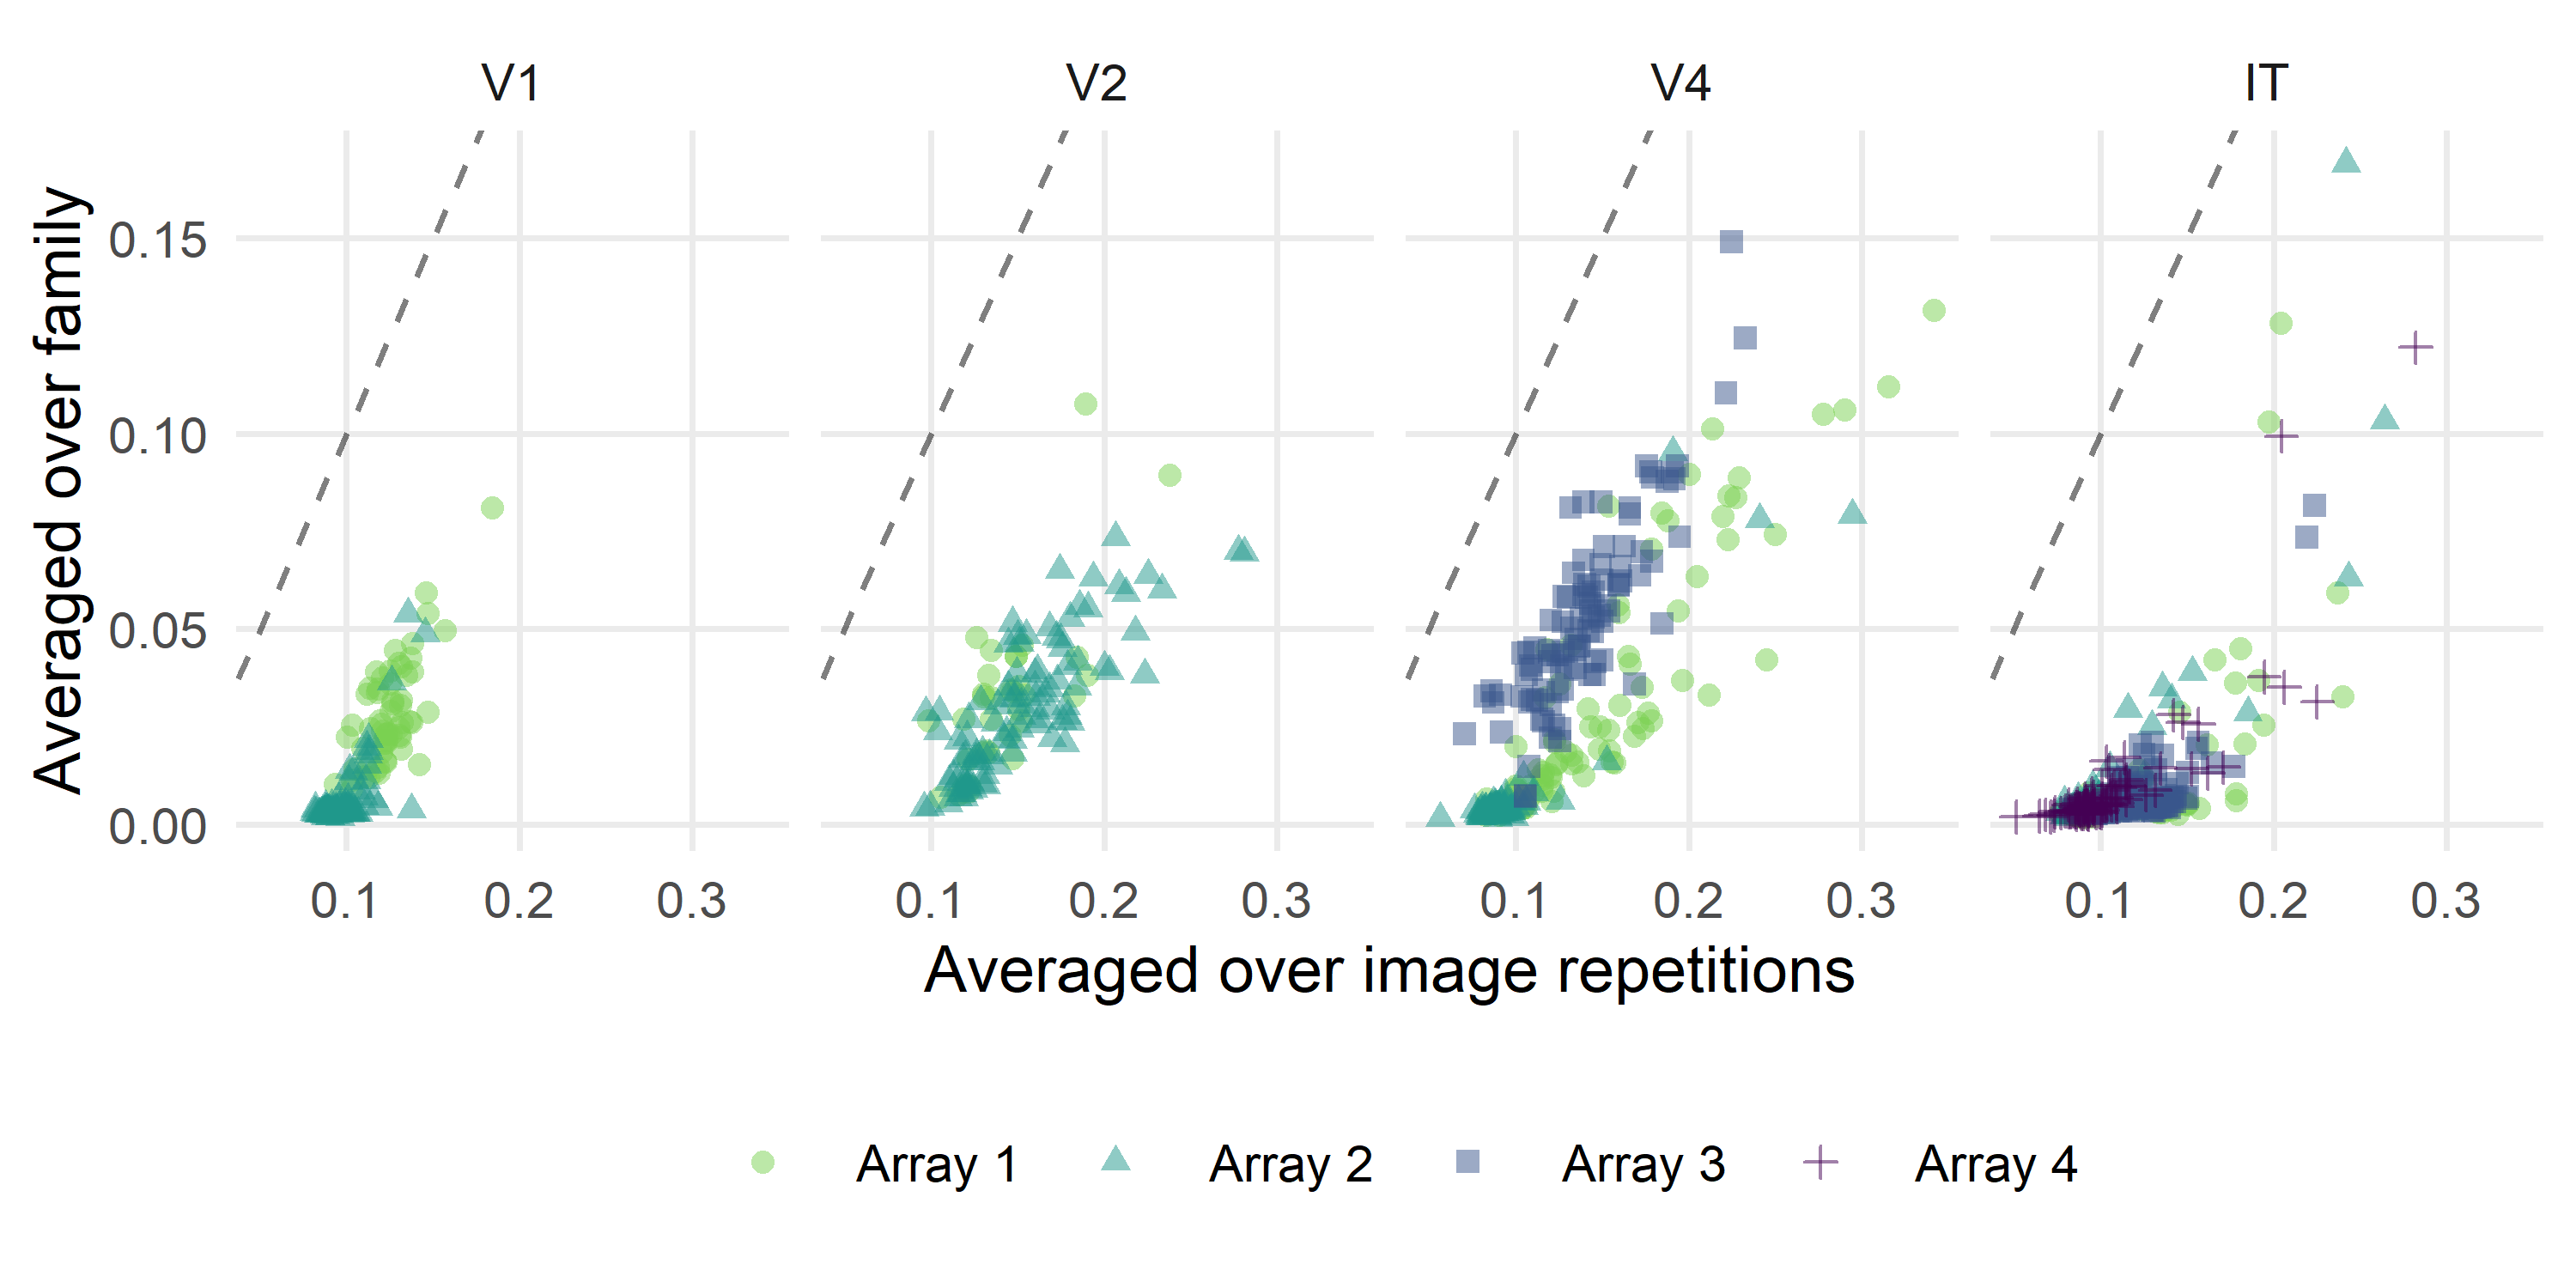
\includegraphics[width=0.8\linewidth]{img/sparsity_fam_vs_img.png}
    \caption{In V1, V2, and V4, lifetime sparsity calculated on image-averaged responses positively correlates with lifetime sparsity calculated on family-averaged responses. In IT, family-averaged responses show low sparsity (high uniformity).}
    \label{fig:sparsity_fam_vs_img}
\end{figure}

\subsection{IT produces informative inhibitory responses to texture stimuli}

\todo{TODO. Likely an Appendix.}

\subsection{Between-family comparisons}

\begin{todoblock}
(TODO: Currently still running the full simulation set for repeated sub-sampling). For now, let's take a somewhat arbitrary ``matched-reliability'' criteria of sites with split-half correlation between \( \rho \in [0.3, 0.6] \), chosen due to similarity of the slopes in the eCDF (Fig. \ref{fig:split_corrs_distribution}). This yields 39 sites in V1, 49 sites in V2, 57 sites in V4, and 53 sites in IT. Figure \ref{fig:dM_pf} shows the results from a single arbitrary subsample of 30 sites from each region alongside the split-half correlations for each site for reference. The distributions for the split-half correlations for the selected sites are not exactly matched, but the trend in reliability does not appear to explain the trend in the distances.
\end{todoblock}

\begin{figure}
    \centering
    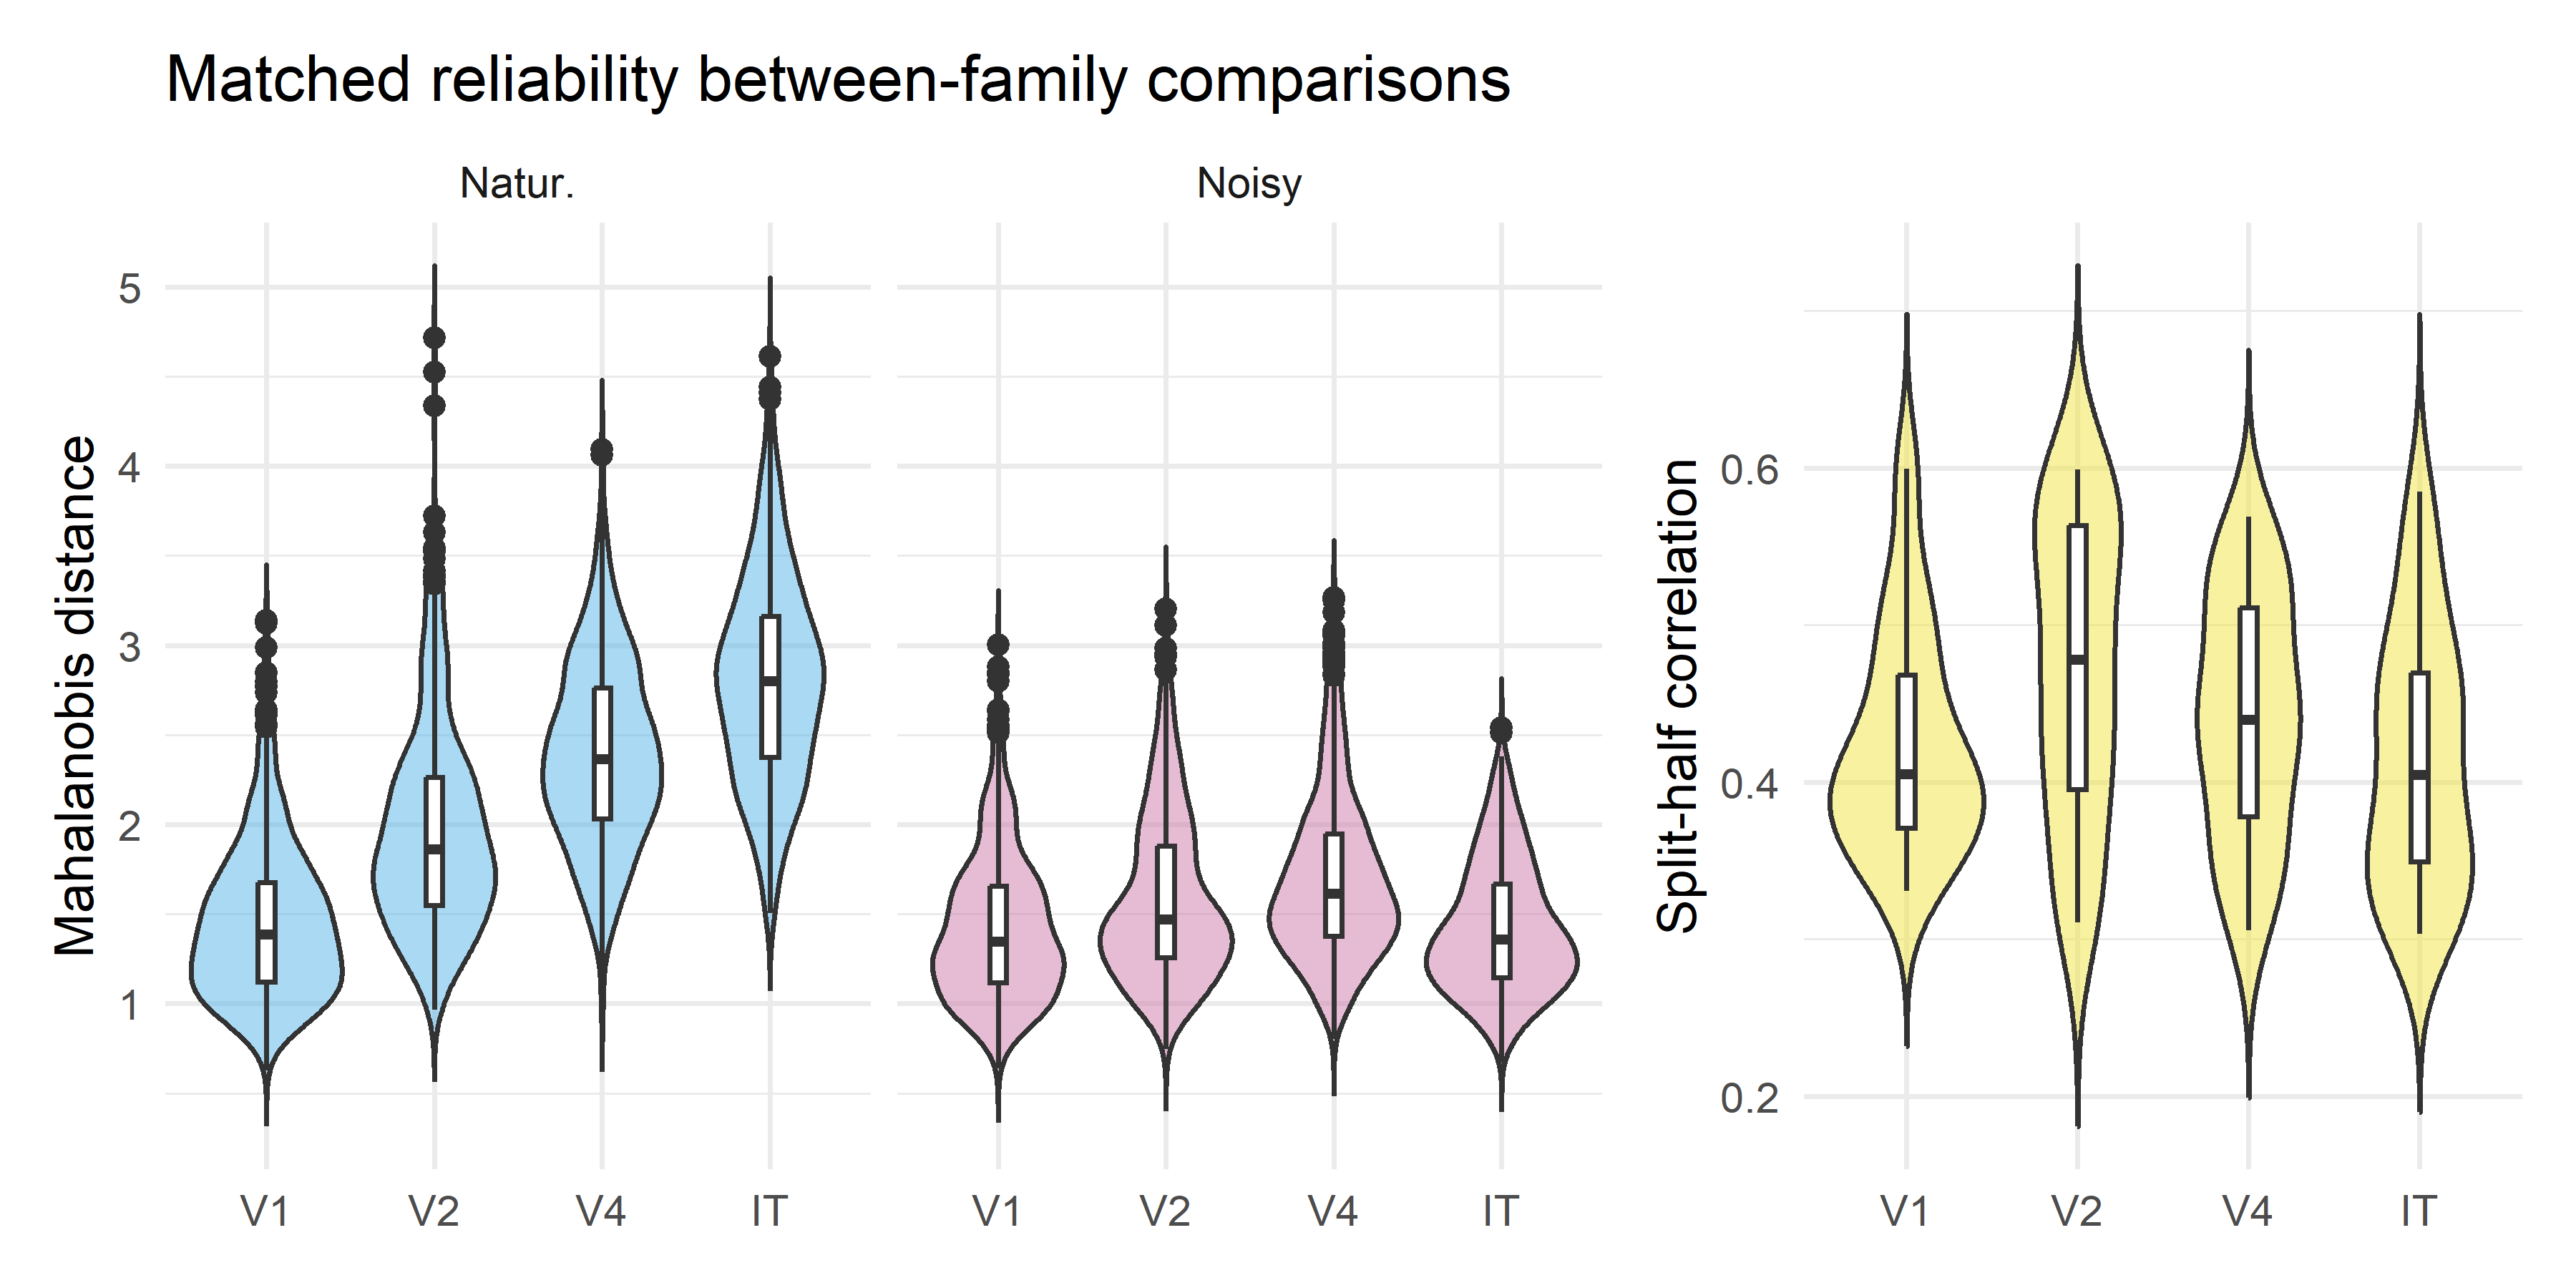
\includegraphics[width=\linewidth]{img/dM_pf.png}
    \caption{(Left) Violin plots of the pairwise between-family Mahalanobis distances, showing a trend of increasing distance with higher visual areas. The plots for noisy textures are included for a comparison, showing noisy distances tend to be shorter with a less pronounced trend. (Right) The split-half correlations of the sites included in the left violin plots show differences in distributions between regions. However, the trends in these distributions do not seem to be aligned with the trends in the naturalistic Mahalanobis distances.}
    \label{fig:dM_pf}
\end{figure}

\subsection{Between-sample (within-family) comparisons}

Figure \ref{fig:dM_ps} is the between-sample analogue to Figure \ref{fig:dM_pf} and shows the results from a single arbitrary subsample of 30 sites from each region alongside the split-half correlations for each site for reference. The site distributions of plit-half correlations are identical to \ref{fig:dM_pf}. Unlike the between-family comparisons, the Mahalanobis distances look similar between naturalistic and noisy texture stimuli. 

\begin{todoblock}
(Need to comb through any interesting family-separated results, such as families with high IT separation.)
\end{todoblock}

\begin{figure}
    \centering
    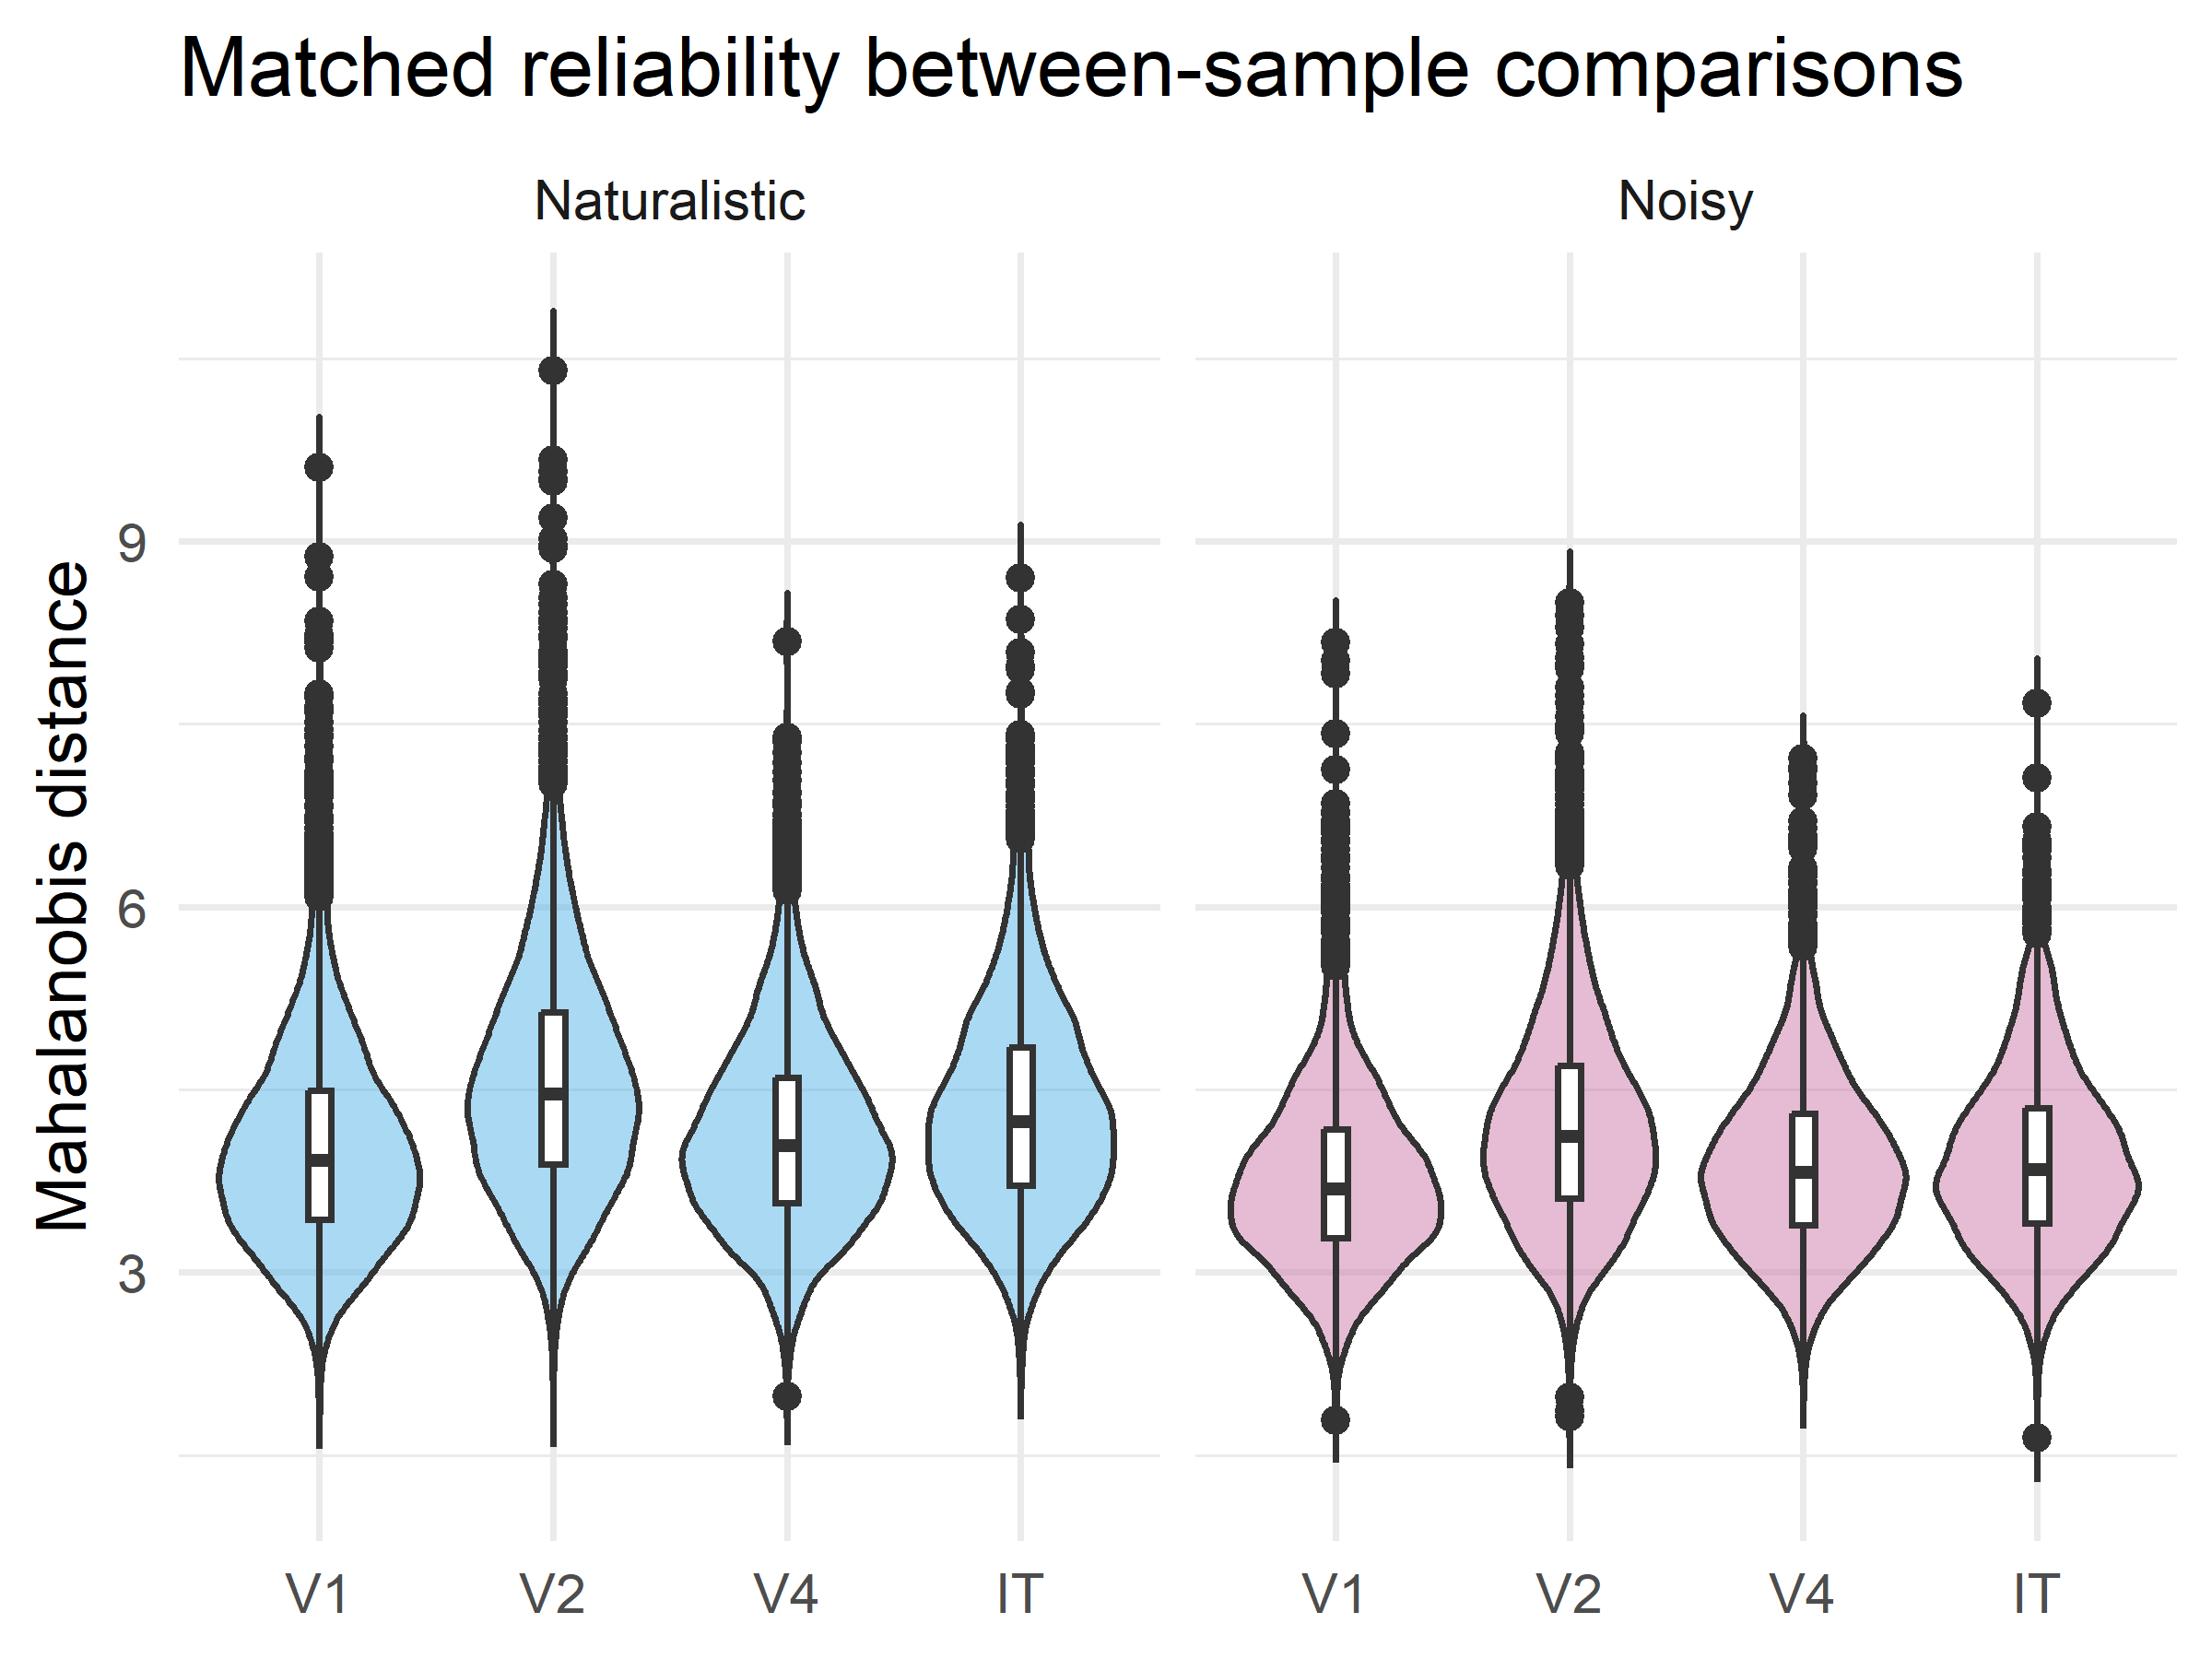
\includegraphics[width=0.6\linewidth]{img/dM_ps.png}
    \caption{Violin plots of the pairwise between-sample Mahalanobis distances, with no obvious trend between regions. The naturalistic and noisy distances appear similar.}
    \label{fig:dM_ps}
\end{figure}
\section{Discussion}

\subsection{IT encodes texture family and sample}

\begin{todoblock}
Figure \ref{fig:dM_pf} suggests that IT sites remain useful for differentiating between texture families and, for certain families, between specific sample images. Though summarization of image statistics may occur in higher regions, the loss of between-sample separability in IT may also be explained by sparse encoding and insufficient sampling of sites. 

These results are sensitive to the choice of reliability. Due to high population and lifetime sparseness of IT sites, performing split-half correlation on family-averaged responses penalizes sparse but informative IT sites and favors favors uniformly weakly responding IT sites (data not yet cleaned). Thus, with a family-averaged reliabilty criteria, IT separability appears lower than V4 (not yet cleaned, probably appendix). 
\end{todoblock}

\subsection{Disagreement with previous findings in V1 and V2}

\begin{todoblock}
Unlike Ziemba et al. (2018) \cite{ziemba_contextual_2018}, we did not find better between-sample discrimination in V1 compared to V2. However, this disagreement may be a feature of the recording quality. For instance, Ziemba et al. performed experiments in anesthetized monkeys. For conscious passive fixation, the receptive fields of V1 neurons may be more misaligned between repetitions. Furthermore, of the two arrays implanted in V1, the array on the border of V1 and V2 contained far more reliable sites. Thus, the most reliable V1 sites may also be sites that are unusually similar to V2.

Furthermore, since data only exist as multi-unit activations, the sparseness of sites may not be accurately captured by our analyses. Receptive fields increase in size in higher regions, so the recorded data from IT likely capture firing from correlated neurons. In contrast, electrode in V1 may be recording from more decorrelated neurons. So, even if individual neurons are sparse and thus more readily decodeable, the summed activity may appear more uniform. 
\end{todoblock}

\subsection{Generalization of results to test data}

\begin{todoblock}
Due to the population sparsity of V1 and IT responses, we did not create a holdout set nor did we perform analyses with particular attention to generalization. Prior work on V1 and V2, such as Ziemba et al. (2018) \cite{ziemba_contextual_2018}, may serve as viable test sets for our findings. However, high-quality experimental data from texture stimuli in IT remain rare, and it may be challenging to perform test analyses for V4 and IT comparisons.
\end{todoblock}

\subsection{Relationship between neural and behavioral discriminability}

\begin{todoblock}
In addition to passive fixation recordings, Lee et al. also measured behavioral sensitivities with a four-choice oddity task. It would be worth investigating whether exposure to the behavioral task changes the between-family and within-family distances. Furthermore, since each region has different maximally separable families, we want to examine which region shows the most alignment to behavioral results.
\end{todoblock}

\newpage

\bibliography{refs}

\newpage

\appendix

\section{Neural data processing details}
\label{appx:preprocessing}

\subsection{Onset time calculation}
\label{appx:onsets}

The criteria for onset time identification is somewhat strict, requiring that \(d'_i (t) \) between non-blank and blank images exceeds a magnitude of 0.4 for three consecutive windows (keeping the sign consistent). Thus, an onset time does not necessarily exist for all sites. IT has the lowest absolute number and lowest proportion of sites with valid onset times, likely due to sparsity. As expected, onset times seem to get longer with higher visual areas. Figure \ref{fig:onsets} contains histograms for the detected onset times. Each region contains a few sites with abnormally long latencies close to 150 ms (recall that the stimulus is presented for 100 ms followed by a 100 ms blank), which are likely spurious. Removing these long latencies did not affect the calculated median onsets. 

\begin{figure}
    \centering
    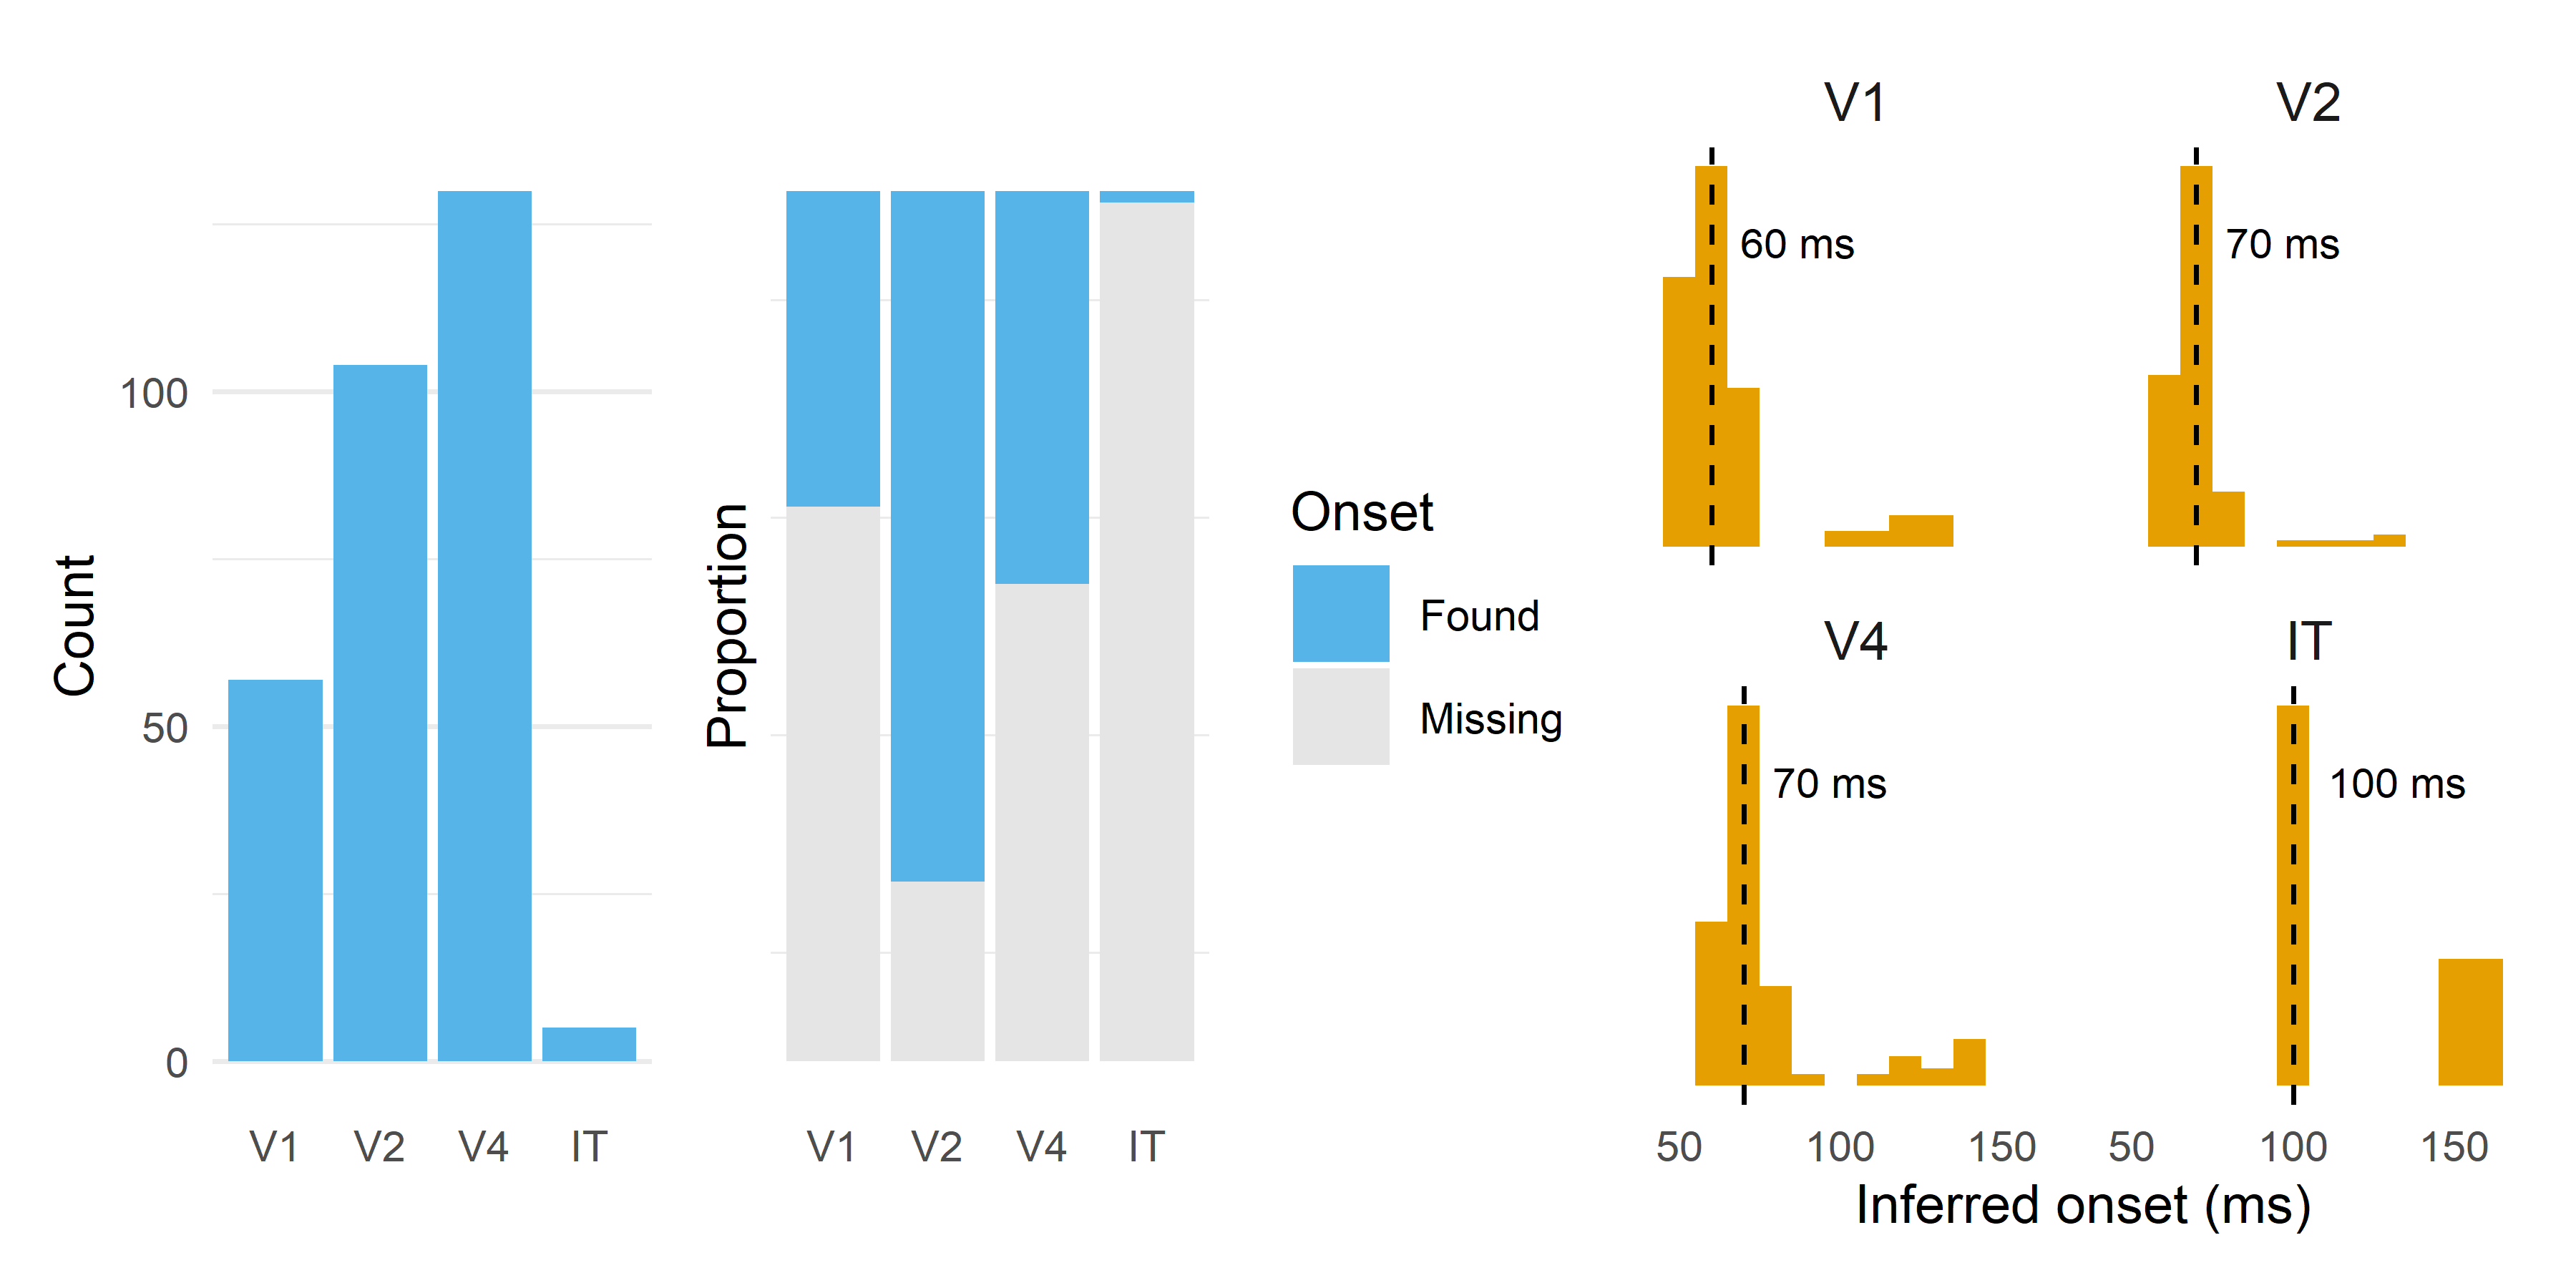
\includegraphics[width=0.9\linewidth]{img/onsets.png}
    \caption{(Left) The number of sites with a calculated onset time given the distance threshold, sorted by region, alongside the proportion of sites in each region with a calculated onset time. IT has both the lowest absolute number and lowest proportion of valid onset times. (Right) Histograms of the calculated onset times per region, with normalized bar heights. Median onset times are indicated with a dashed line.}
    \label{fig:onsets}
\end{figure}

\subsection{Split-half correlation}
\label{appx:split_corrs}

We tested split half correlations over all \( \binom{6}{3} = 20 \) possible splits of the six repetitions of the images. For all regions, we found small standard deviation for split-half correlations over different splits. The mean standard deviation fell between 0.01 and 0.02, and the maximum between 0.03 to 0.04.

When calculating split-half correlations, the blank stimuli can be: 1) \textbf{separated} into averages within 100 groups based on the ``repetition'' of blanks in each repetition round of stimuli, 2) \textbf{aggregated} over all blank stimuli into one overall average, or 3) \textbf{omitted} entirely. The handling of the blank images did not produce a large difference in the observed correlations (Fig. \ref{fig:split_corrs_blanks}). We defaulted to the single aggregated blank group. 

\begin{figure}
    \centering
    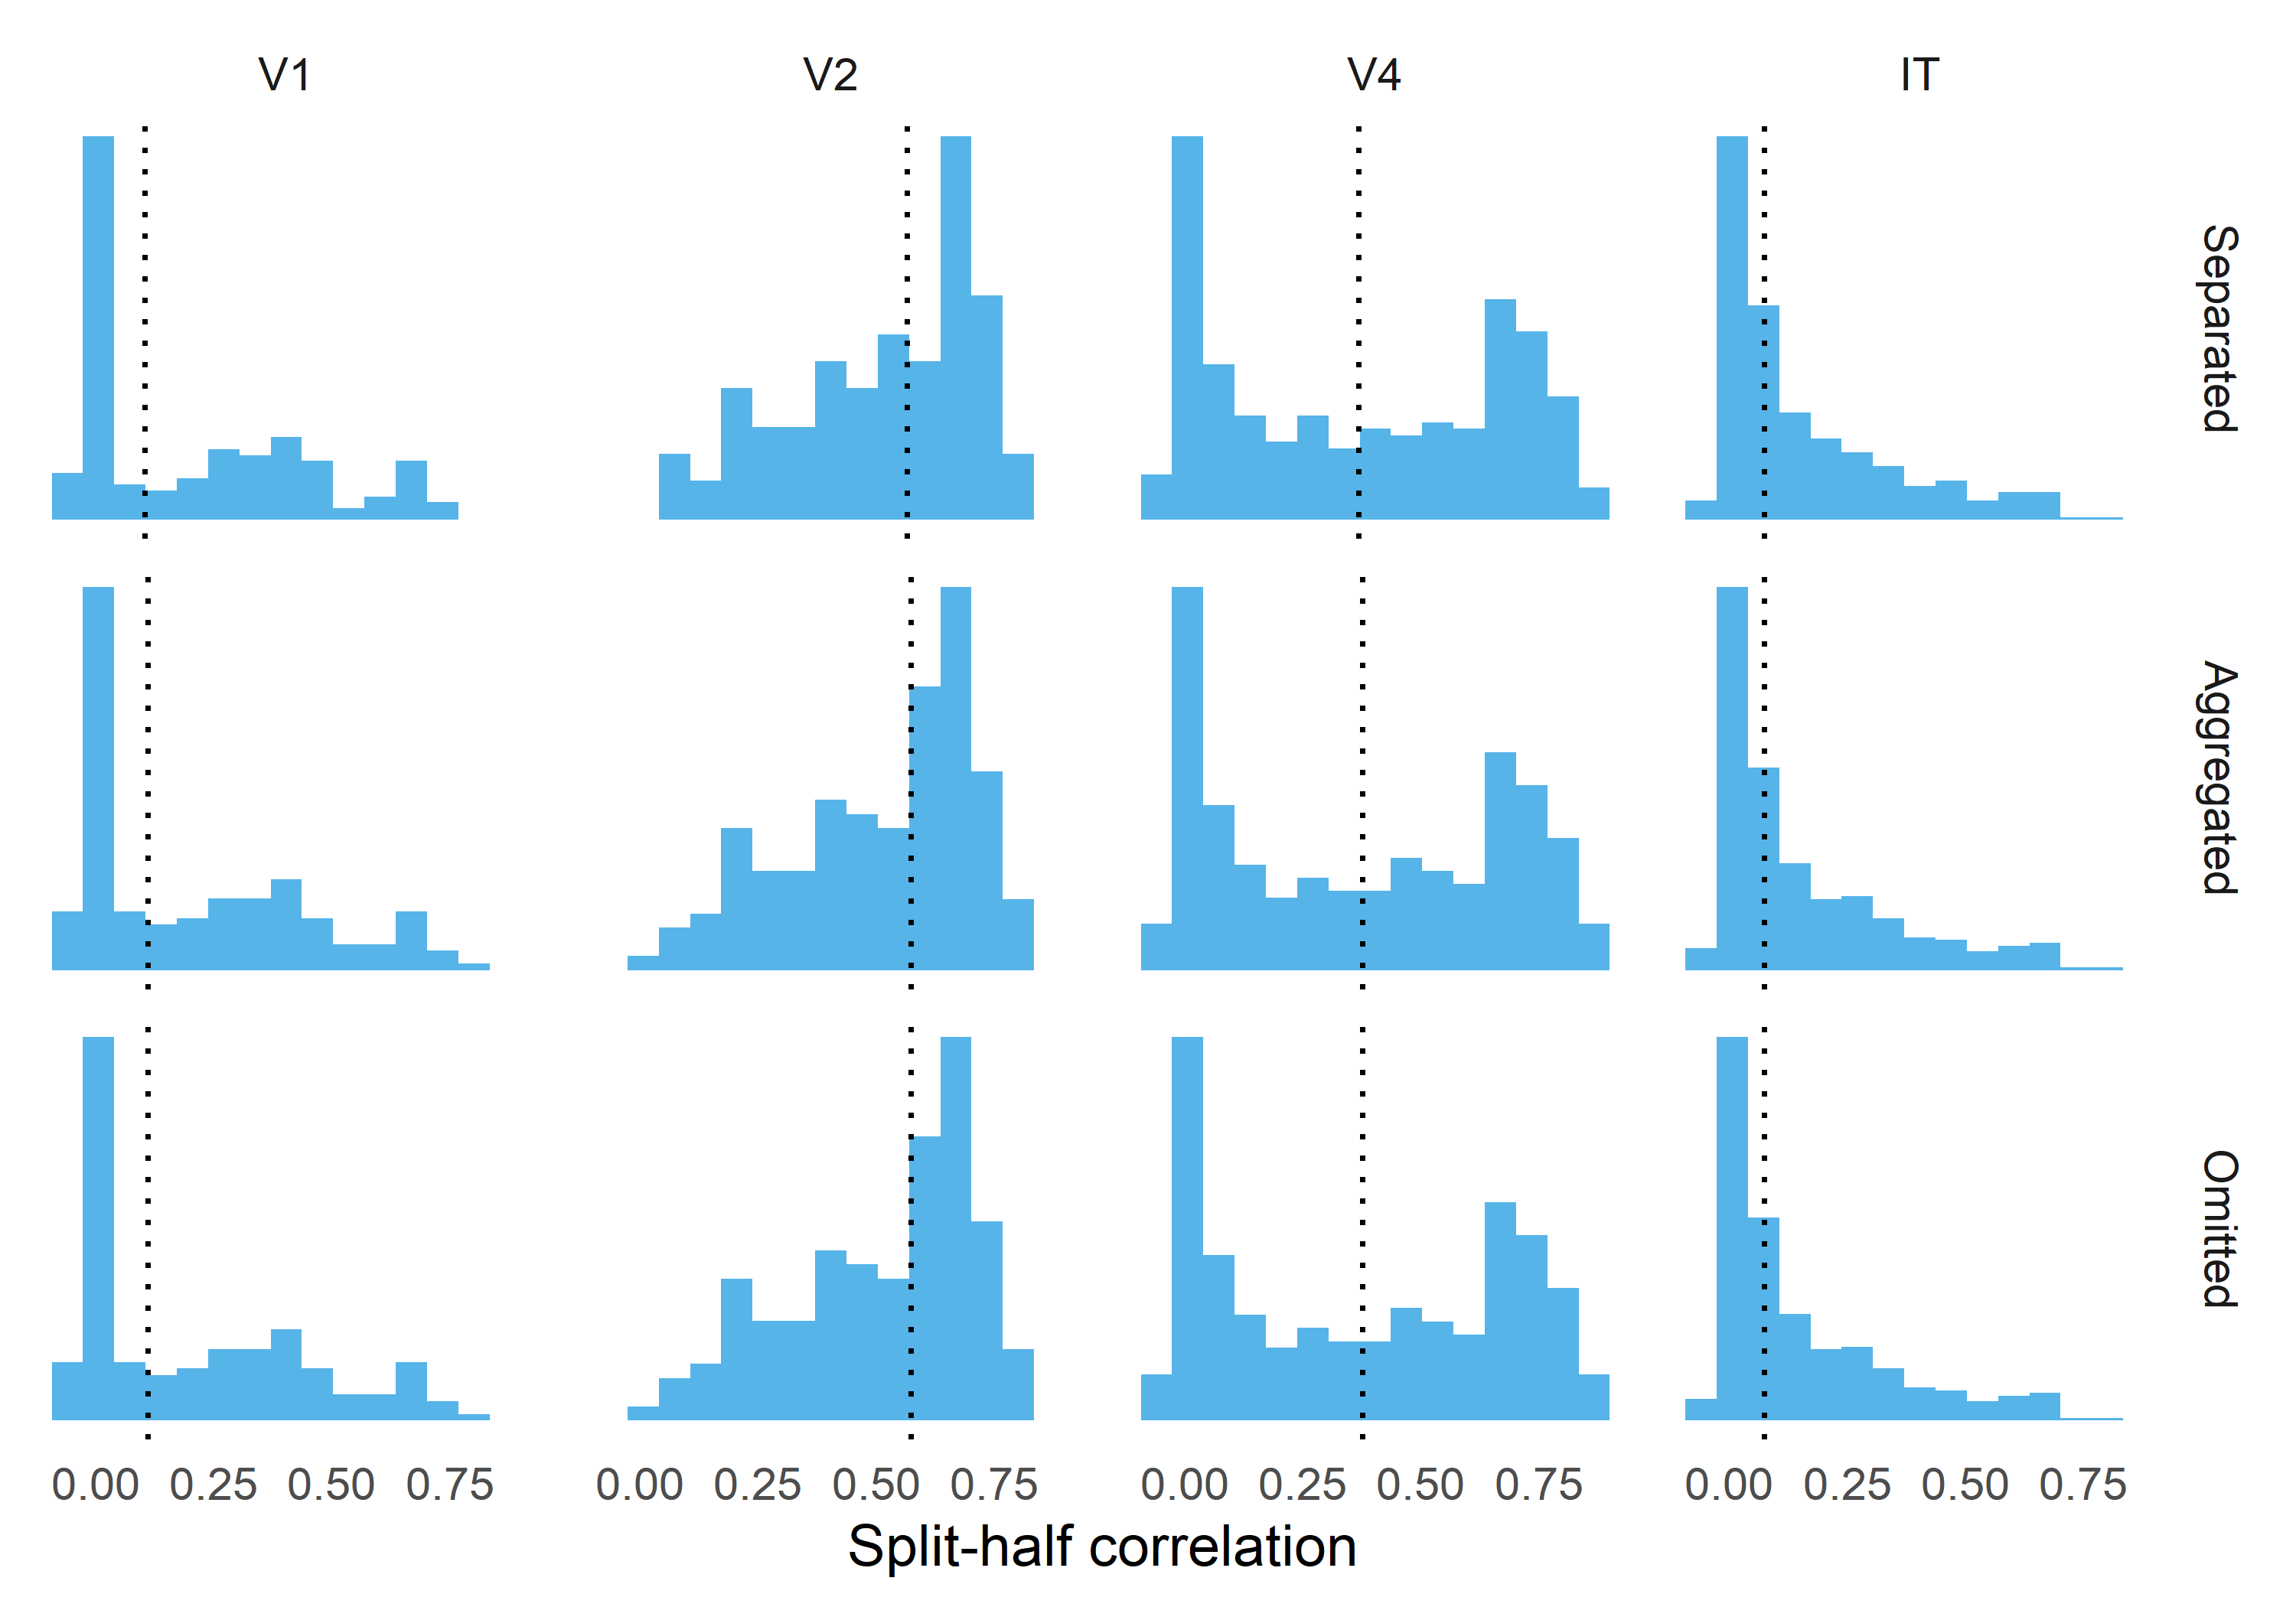
\includegraphics[width=0.8\linewidth]{img/split_corrs_blanks.png}
    \caption{Normalized histograms of the split-half correlations calculated for each site, averaged across the 20 possible splits. The rows indicate the handling of blank images included in the vectors used for the split-half correlation calculation, with blanks either omitted entirely, aggregated over all repetitions, or separated into 100 instances of 6 repetitions each. Dashed lines mark the median. The distribution of correlations for V1 and IT are more right-skewed. Differences between the number of blank images are slight, though in general, the median correlation is lowest when including separated blank images (with the exception of IT).}
    \label{fig:split_corrs_blanks}
\end{figure}

\newpage

\section{Results did not change when shifting the window of averaging}
\label{appx:window}

\newpage

\section{Estimating sparsity}

\subsection{Comparison of sparsity measures}
\label{appx:sparsity} 

For brevity, we will describe various measures of sparsity with reference to lifetime sparsity for a single fixed site \( s \). Let stimuli be indexed from \( i = 1, \dots, n \) and let \(\mu_{i} \geq 0 \) be site \( s \)'s response to the \(i\)th stimulus. 

Hurley and Rickard (2009) describe six desiderata of a sparsity metric, based on literature on income inequality \cite{hurley_comparing_2009}. A measure of sparsity should

\begin{enumerate}
    \item decrease if the distance between the highest and lowest responses decreases (``Robin Hood''),
    \item be invariant to a uniform scaling of the responses,  
    \item decrease if a positive constant is added to each response, 
    \item be invariant to duplication of the responses,
    \item increase if one response grows large, and  
    \item increase if many zero responses are added to the set. 
\end{enumerate}

Among the sparsity measures they consider, Hurley and Rickard prove that only the Gini index and \( pq \)-mean sparsity fulfill all six criteria. For ordered responses \( \mu_{s, (1)} \leq \mu_{s, (2)} \leq \cdots \leq \mu_{s, (n)}, \) the Gini index can be calculated as 
\[ 
% S_{\textrm{Gini}} = 
% \frac{2}{n^2 \overline{r}}
% \sum_{i = 1}^n i \left( \mu_{(i)} - \overline{\mu} \right):  \overline{\mu} = \frac{1}{n} \sum_{i = 1}^{n} \mu_{s, i}.
S_{\textrm{Gini}} = 
1 - \frac{2}{n \sum_{i = 1}^n \mu_{s, i}} \sum_{i = 1}^n
\mu_{s, (i)} \left( n - i + 1/2 \right). \]
The \(pq\)-mean can be found as the ratio of generalized means
\[ 
S_{pq} = - \frac{\left( \frac{1}{n} \sum_{i = 1}^n \mu_{s, i}^p \right)^{1 / p}}{\left( \frac{1}{n} \sum_{i = 1}^n \mu_{s, i}^q \right)^{1/q}},
\]
and satisfies the desiderata when \( p \leq 1, q > 1 \). 

For \( p = 1, q = 2 \), the \( pq \)-mean sparsity resembles the ratio of the first and second moments (RM), a common sparseness measure in neuroscience \cite{rolls_sparseness_1995, vinje_sparse_2000}. The RM sparsity can be found as
\begin{equation}
S_{\textrm{RM}} = \left( 1 - \frac{\left( \frac{1}{n} \sum_{i = 1}^n \mu_{i} \right)^2}{\frac{1}{n} \sum_{i = 1}^n \mu_{i}^2} \right) \left( \frac{1}{1 - \frac{1}{n}} \right).
\end{equation}
In the above formula, the term \( \left( \frac{1}{1 - \frac{1}{n}} \right) \) scales the above to \( [0, 1] \), with 0 indicating uniformity and 1 indicating maximal concentration. However, the above does not meet desiderata (4). 

\textit{Aside}: In general, scaling to improve interpretability trades off with invariance to duplication. For example, in the extreme case with only a single non-zero response, \( S_{\textrm{Gini}} = \frac{n - 1}{n} \). Thus, a common correction scales the Gini index by \( \frac{n}{n - 1} \) such that \( 1 \) indicates maximum concentration in the data, and the resulting measure no longer satisfies desiderata (4).

In neural response separability, one might be interested in responses relative to the site's baseline rather than zero. Let \( \mu_{s, 0} \) be the baseline response for site \( s \), defined as the mean response to blank stimuli.
%Consider a site with a baseline response of 60 Hz where most of the stimuli produce an average response of 61 Hz while a single stimulus produces an average response of 80 Hz. Should this be measured as the same sparsity as a site with a baseline of 10 Hz, most stimuli evoking 11 Hz, and a single stimulus evoking 30 Hz? Furthermore, what about a site with a baseline of 60 Hz, most stimuli evoking 59 Hz, and a single stimulus at 40 Hz? 
We experimented with a few different strategies: 

\begin{enumerate}
    \item calculating sparsity with respect to \( \mu_{s, i} \), ignoring the baseline; 
    \item subtracting the baseline, i.e., \( \mu_{s, i} - \mu_{s, 0} \); or
    \item taking the log ratio, i.e., \( \log_2 \left( \mu_{s, i} / \mu_{s, 0} \right). \)
\end{enumerate}

When correcting for baseline firing, note that many common sparsity measures (including the Gini index, \( pq \)-mean, and RM) cannot be applied to a mix of positive and negative values. As an alternative, we can apply the Hoyer sparsity measure \cite{hoyer_non-negative_2004}, defined as
\[ 
S_{\textrm{Hoyer}} = \frac{1}{\sqrt{n} - 1} \left( \sqrt{n} - \frac{\sum_{i = 1}^n |\mu_{s, i}|}{\sqrt{\sum_{i = 1}^n \mu_{s, i}^2}} \right).
\]
Like \( S_{\textrm{RM}}\), \( S_{\textrm{Hoyer}} \) is bounded by \( [0, 1] \), with 0 indicating complete uniformity and 1 indicating a single non-zero value. Similarly, \( S_{\textrm{Hoyer}} \) fulfills Hurley and Rickard's listed desiderata, with the exception of (4) \cite{hurley_comparing_2009}. Outside of \( S_{\textrm{Hoyer}} \), one can simply apply the standard sparsity measures to the absolute value of the transformed responses. 

\subsection{Different sparsity metrics produce similar results}
\label{appx:sparsity_vs}

\newpage

\section{Handling wide data in between-sample comparisons}

\subsection{Sketch of shrinkage covariance estimation}
\label{appx:shrinkage}

To briefly describe Schafer and Strimmer's derivation \cite{schafer_shrinkage_2005}, let \( \boldsymbol{\psi} = (\psi_1, \dots, \psi_p) \) be the parameters of an unrestricted high-dimensional model of interest and let \( \boldsymbol{\theta} \) be the parameters of a lower dimensional restricted sub-model. E.g., \( \boldsymbol{\psi} \) is the mean vector of a multivariate Normal and \( \boldsymbol{\theta} \) is the vector of a contrained submodel where the means are all assumed to be equal. Then, the linear shrinkage approach finds the new estimator
\[ \boldsymbol{\psi}^* = \mu \hat{\boldsymbol{\theta}} + (1 - \mu) \hat{\boldsymbol{\psi}} : \mu \in [0, 1] \]
where the optimal value \( \mu^* \) can be found analytically by optimizing 
\[ \mu^* = 
\frac
{\sum_{i = 1}^p \left( \var (\hat\psi_i) - \cov (\hat\theta_i, \hat\psi_i) \right)}
{\sum_{i = 1}^p \E [(\hat\theta_i - \hat\psi_i)^2]}. \]

In \texttt{corpcor}, the shrinkage target (i.e., the parameters of the constrained model) is taken as a diagonal covariance matrix whose diagonal entries may be unequal, which shrinks the off-diagonal elements of the estimated covariance matrix \cite{schafer_shrinkage_2005, schafer_corpcor_2021}. This also produces a positive definite covariance estimate, as a convex combination of a positive definite matrix and positive semidefinite matrix yields a positive definite matrix. 

\subsection{Comparison with randomized dichotomies}

\begin{todoblock}
Rather than apply shrinkage, the number of samples in the within-family comparisons can be inflated with a randomized dichotomy approach. Two groups of 7 sample IDs each (without replacement) were selected. Because this is not an even split of the available sample IDs, groups were generated with a stratified approach:
\begin{enumerate}
    \item Omit one of the 15 IDs (1, 2, ..., 15). 
    \item Take a random sample of the possible \( \binom{14}{7} \) combos of the remaining indices. 
\end{enumerate}
Then, \( d_M \) calculation can proceed with the non-shrinkage sample covariance estimator. Visually, the distributions between the pairwise sample comparisons and the randomized dichotomies look similar, though the magnitudes of the distances are affected by the different number of samples. When plotting the within-family averages and standard deviations against each other (Fig. \ref{fig:shrinkage_vs_randdichot}), the correlations tend to be good for within-family averages and worse for within-family standard deviations (Table \ref{tbl:shrinkage_vs_randdichot}). To make this more rigorous, one could test for similarity between the relative rankings of region performance with a post hoc test. I am fairly unworried about large differences in the results from the pairwise sample distances and the randomized dichotomies. Thus, analyses proceeded with the pairwise sample distances (with shrinkage), as they tend to be more intuitive. 

\begin{figure}
    \centering
    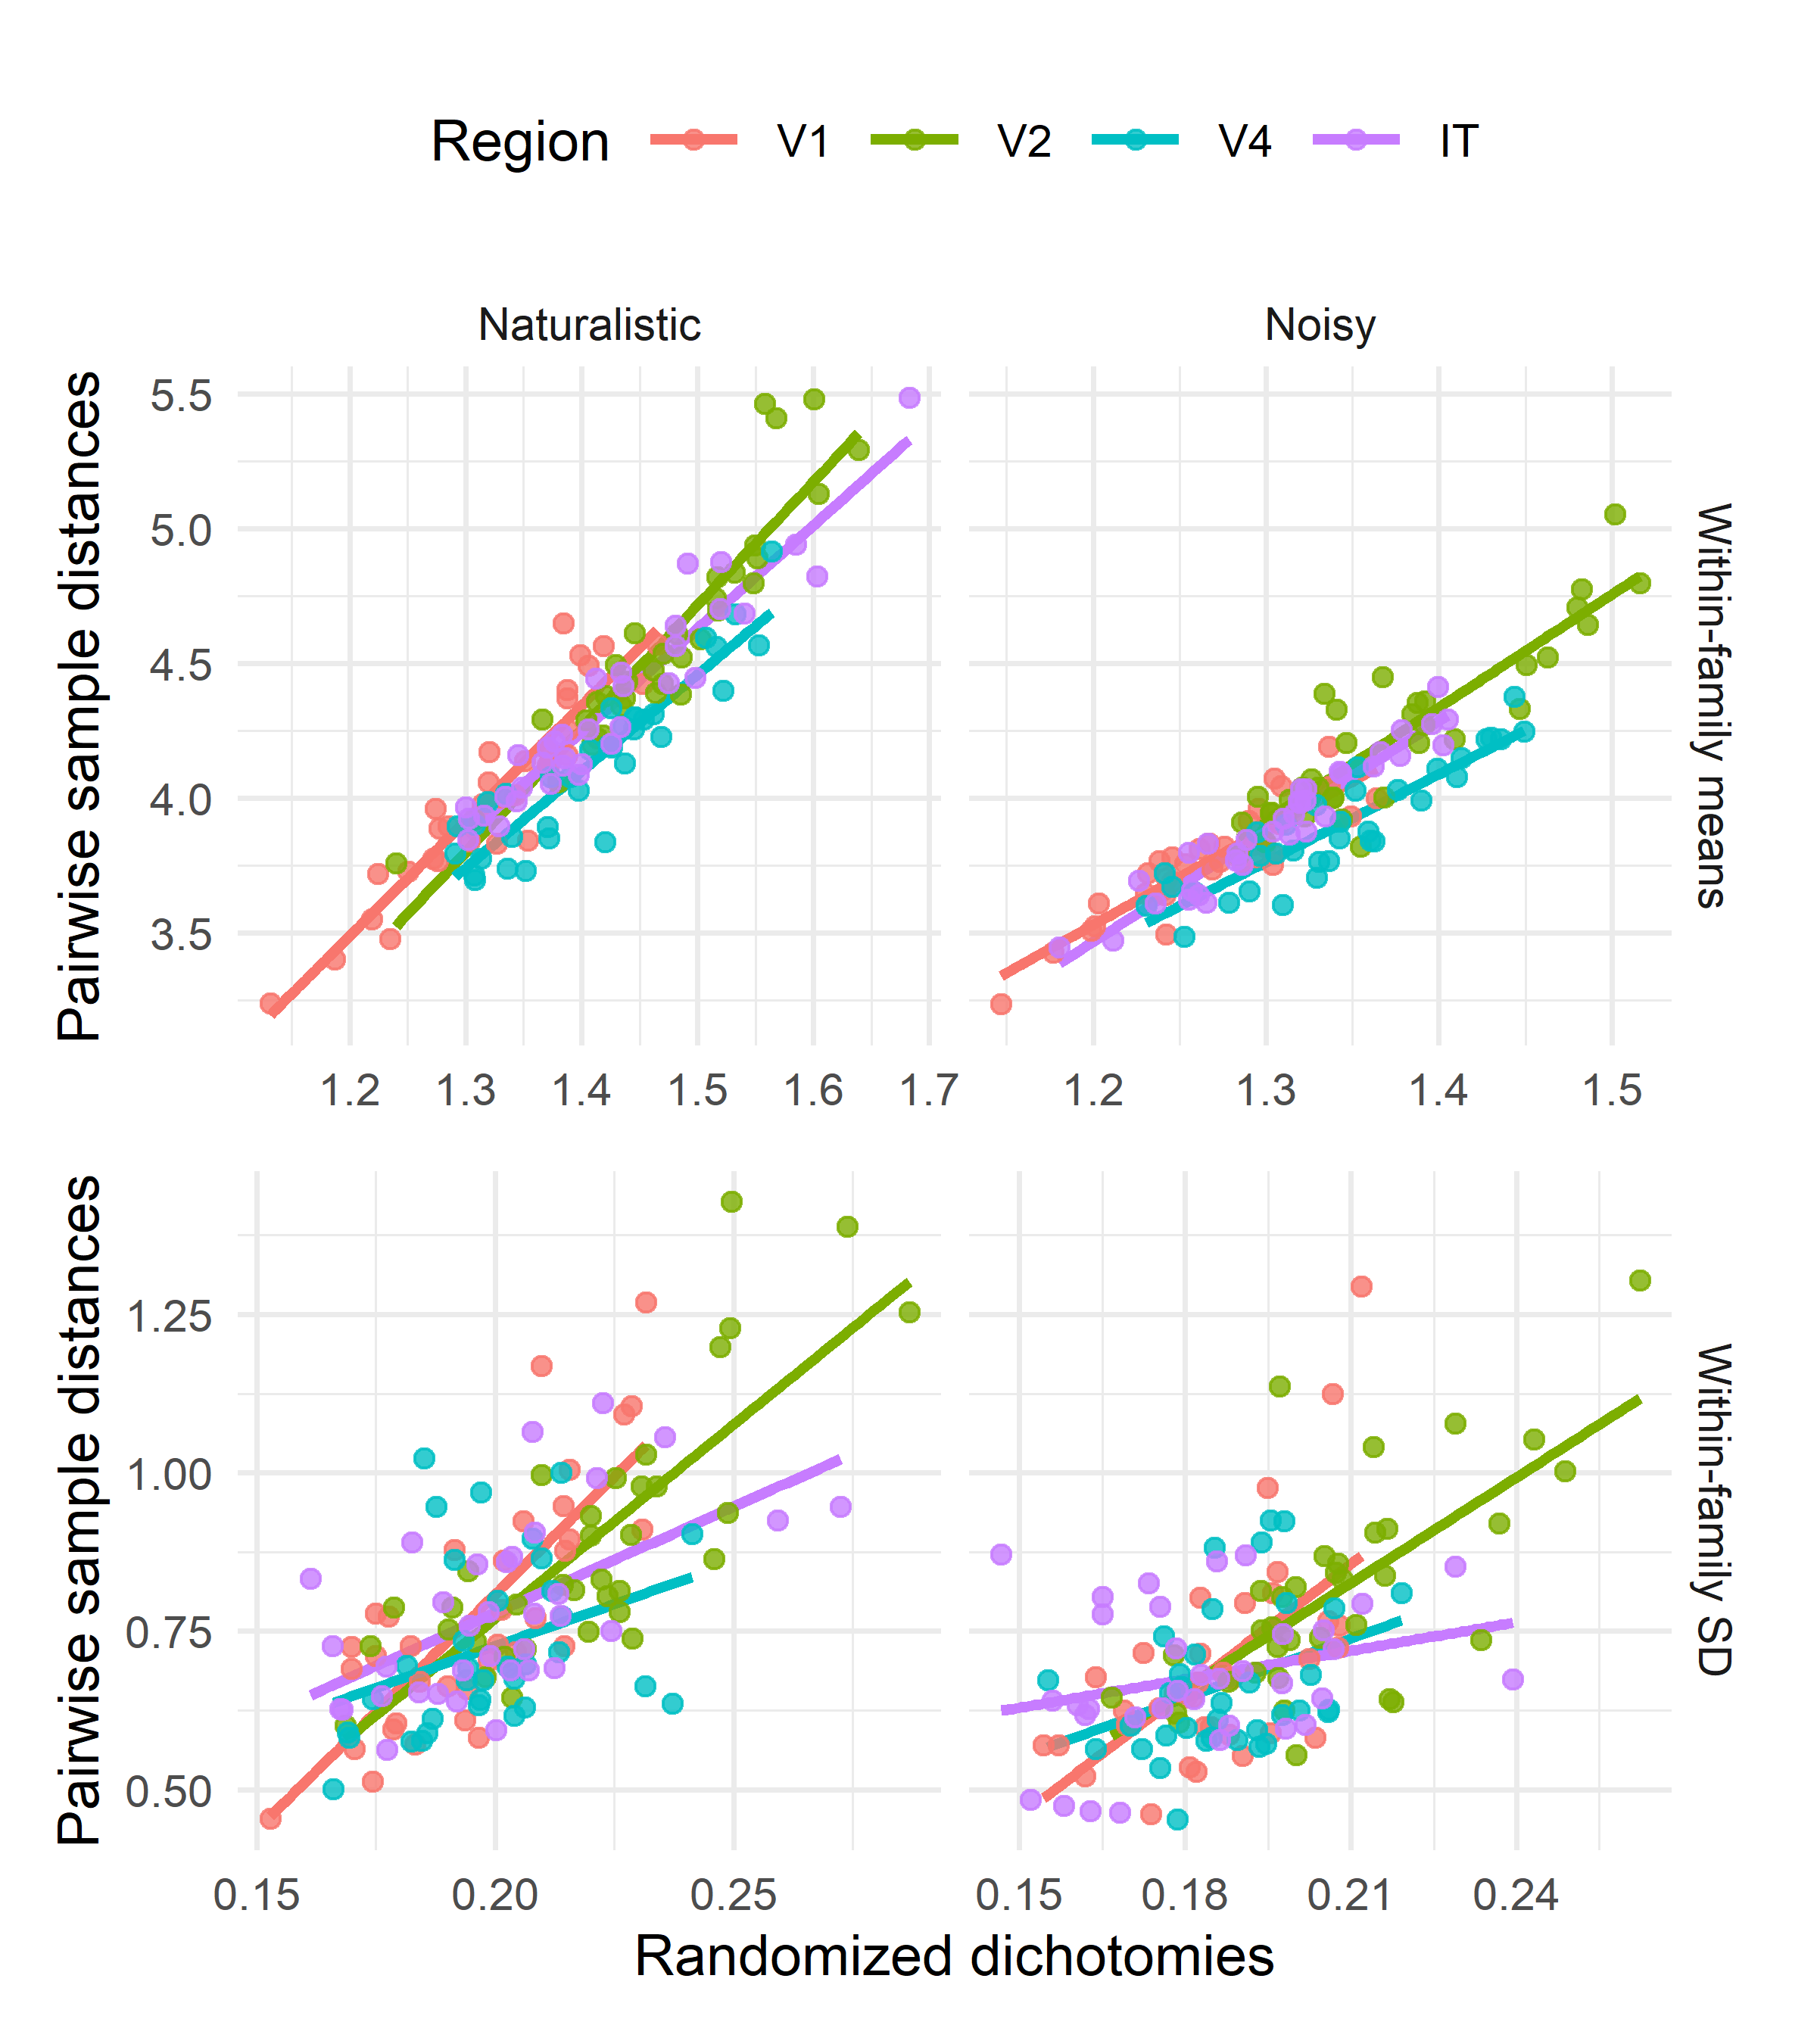
\includegraphics[width=0.7\linewidth]{img/shrinkage_vs_randdichot.png}
    \caption{Means and standard deviations are calculated within each texture family. The within-family means tend to show more correlation across all regions. The correlation between the pairwise sample and randomized dichotomies standard deviations is worse in IT than other regions.}
    \label{fig:shrinkage_vs_randdichot}
\end{figure}

\begin{table}[]
    \centering
    \small
    \begin{tabular}{crrrr}
    \toprule
    ~ & \multicolumn{2}{c}{Naturalistic} & \multicolumn{2}{c}{Noisy} \\
    Region & Corr(Means) & Corr(SD) & Corr(Means) & Corr(SD)  \\
    \midrule
    V1 & 0.929 & 0.785 & 0.892 & 0.592 \\
    V2 & 0.922 & 0.797 & 0.898 & 0.682 \\
    V4 & 0.919 & 0.344 & 0.908 & 0.357 \\
    IT & 0.957 & 0.578 & 0.963 & 0.281 \\
    \bottomrule
    \end{tabular}
    \caption{Correlations for the plots in Figure \ref{fig:shrinkage_vs_randdichot}.}
    \label{tbl:shrinkage_vs_randdichot}
\end{table}

\end{todoblock}
\newpage 


\end{document}
